\section{Results} \label{sec:results}
Several simulations were run with \gls{sispo} in order to assess the capabilities and quality of the output of the three stages, i.e. rendering, compression and reconstruction. Furthermore, the effects of compression using the \gls{jp2} standard on the quality of \gls{3d} model reconstruction.

\subsection{Rendering} \label{sec:results_sim}
A subset of all settings was kept constant for all simulations. The instrument settings are presented in Table \ref{tab:inst_settings} and the settings for the \gls{sssb} in Table \ref{tab:sssb_settings}. The specific values were chosen in order to mimic the scenario in \cite{Pajusalu2019CharacterizationMapping}.

\begin{table}[htb]
    \centering
    \caption{Instrument Settings}
    \label{tab:inst_settings}
    \begin{tabular}{l|l}
        \textbf{Parameter Name} & \textbf{Value} \\ \hline
        res       & $\SI{2464}{} \times \SI{2054}{}$   \\
        pix\_l        & \SI{3.45}{\micro\meter}     \\
        focal\_l       & \SI{230}{\milli\meter}     \\
        aperture\_d     &  \SI{4}{\centi\meter} \\
        wavelength  & \SI{550}{\nano\meter} \\
        quantum\_eff & \SI{0.25}{} \\
        color\_depth & \SI{8}{\bit}
    \end{tabular}
\end{table}

\begin{table}[htb]
    \centering
    \caption{\gls{sssb} settings.}
    \label{tab:sssb_settings}
    \begin{tabular}{l|l}
        \textbf{Parameter Name} & \textbf{Value} \\ \hline
        a       & \SI{1.644641475071416}{\astronomicalunit}   \\
        e        & \SI{3.838774437558215E-01}{}\\
        i       & \SI{3.408231185574551E+00}{\radian}\\
        P &  \SI{7.703805051391988E+02}{\radian} \\
        omega  & \SI{3.192958853076784E+02}{\radian} \\
        Omega & \SI{7.320940216397703E+01}{\radian} \\
        M & \SI{1.967164895190036E+02}{\radian} \\
        date & 2017-08-19T00:00:00.000 \\
        rotation\_rate & \SI{8133.48}{\per\second} \\
        albedo & \SI{0.15}{} \\
        max\_dim & \SI{512}{}
    \end{tabular}
\end{table}

\begin{table}[htb]
    \centering
    \caption{Simulation settings.}
    \label{tab:sim_settings}
    \begin{tabular}{l|l}
        \textbf{Parameter Name} & \textbf{Value} \\ \hline
        duration       & \SI{120}{\second}   \\
        encounter\_date & 2017-08-15T12:00:00.000\\
        frames       & \SI{120}{}     \\
        relative\_velocity     &  \SI{10}{\kilo\meter\per\second} \\
        with\_terminator  & \SI{0}{} \\
        with\_sunnyside & \SI{1}{} \\
        timesampler\_mode & \SI{1}{} \\
        exposure & \SI{0}{} \\
        samples & \SI{48}{} \\
        device & \gls{gpu} \\
        tile\_size & \SI{512}{} \\
        with\_clipping & \SI{1}{}
    \end{tabular}
\end{table}

\subsubsection{Image Comparison}
In a first step, the overall image quality is compared visually to real images. A set of images at different distances of nuclei with different sizes is depicted in Figure \ref{fig:render_quali_comparison}. A set of five images from asteroid Bennu taken by the PolyCam aboard the \textit{OSIRIS-REx} mission is shown in Figure \ref{fig:render_quali_bennu}. Additionally, the rendered images are compared to images of comet \gls{67p} taken by the OSIRIS imager aboard the \textit{Rosetta} spacecraft. Figure \ref{fig:render_quali_67p} shows one image that represents all important features of \gls{67p}. A collection of several views of the comet \gls{81p}, also known as Wild 2, are shown in Figure \ref{fig:render_quali_81p}. \Gls{81p} was visited during the \textit{Stardust} mission \cite{Brownlee2003Stardust:Mission}.

\begin{figure}[htb]
    \centering
        \begin{subfigure}[b]{0.48\textwidth}
            \centering
                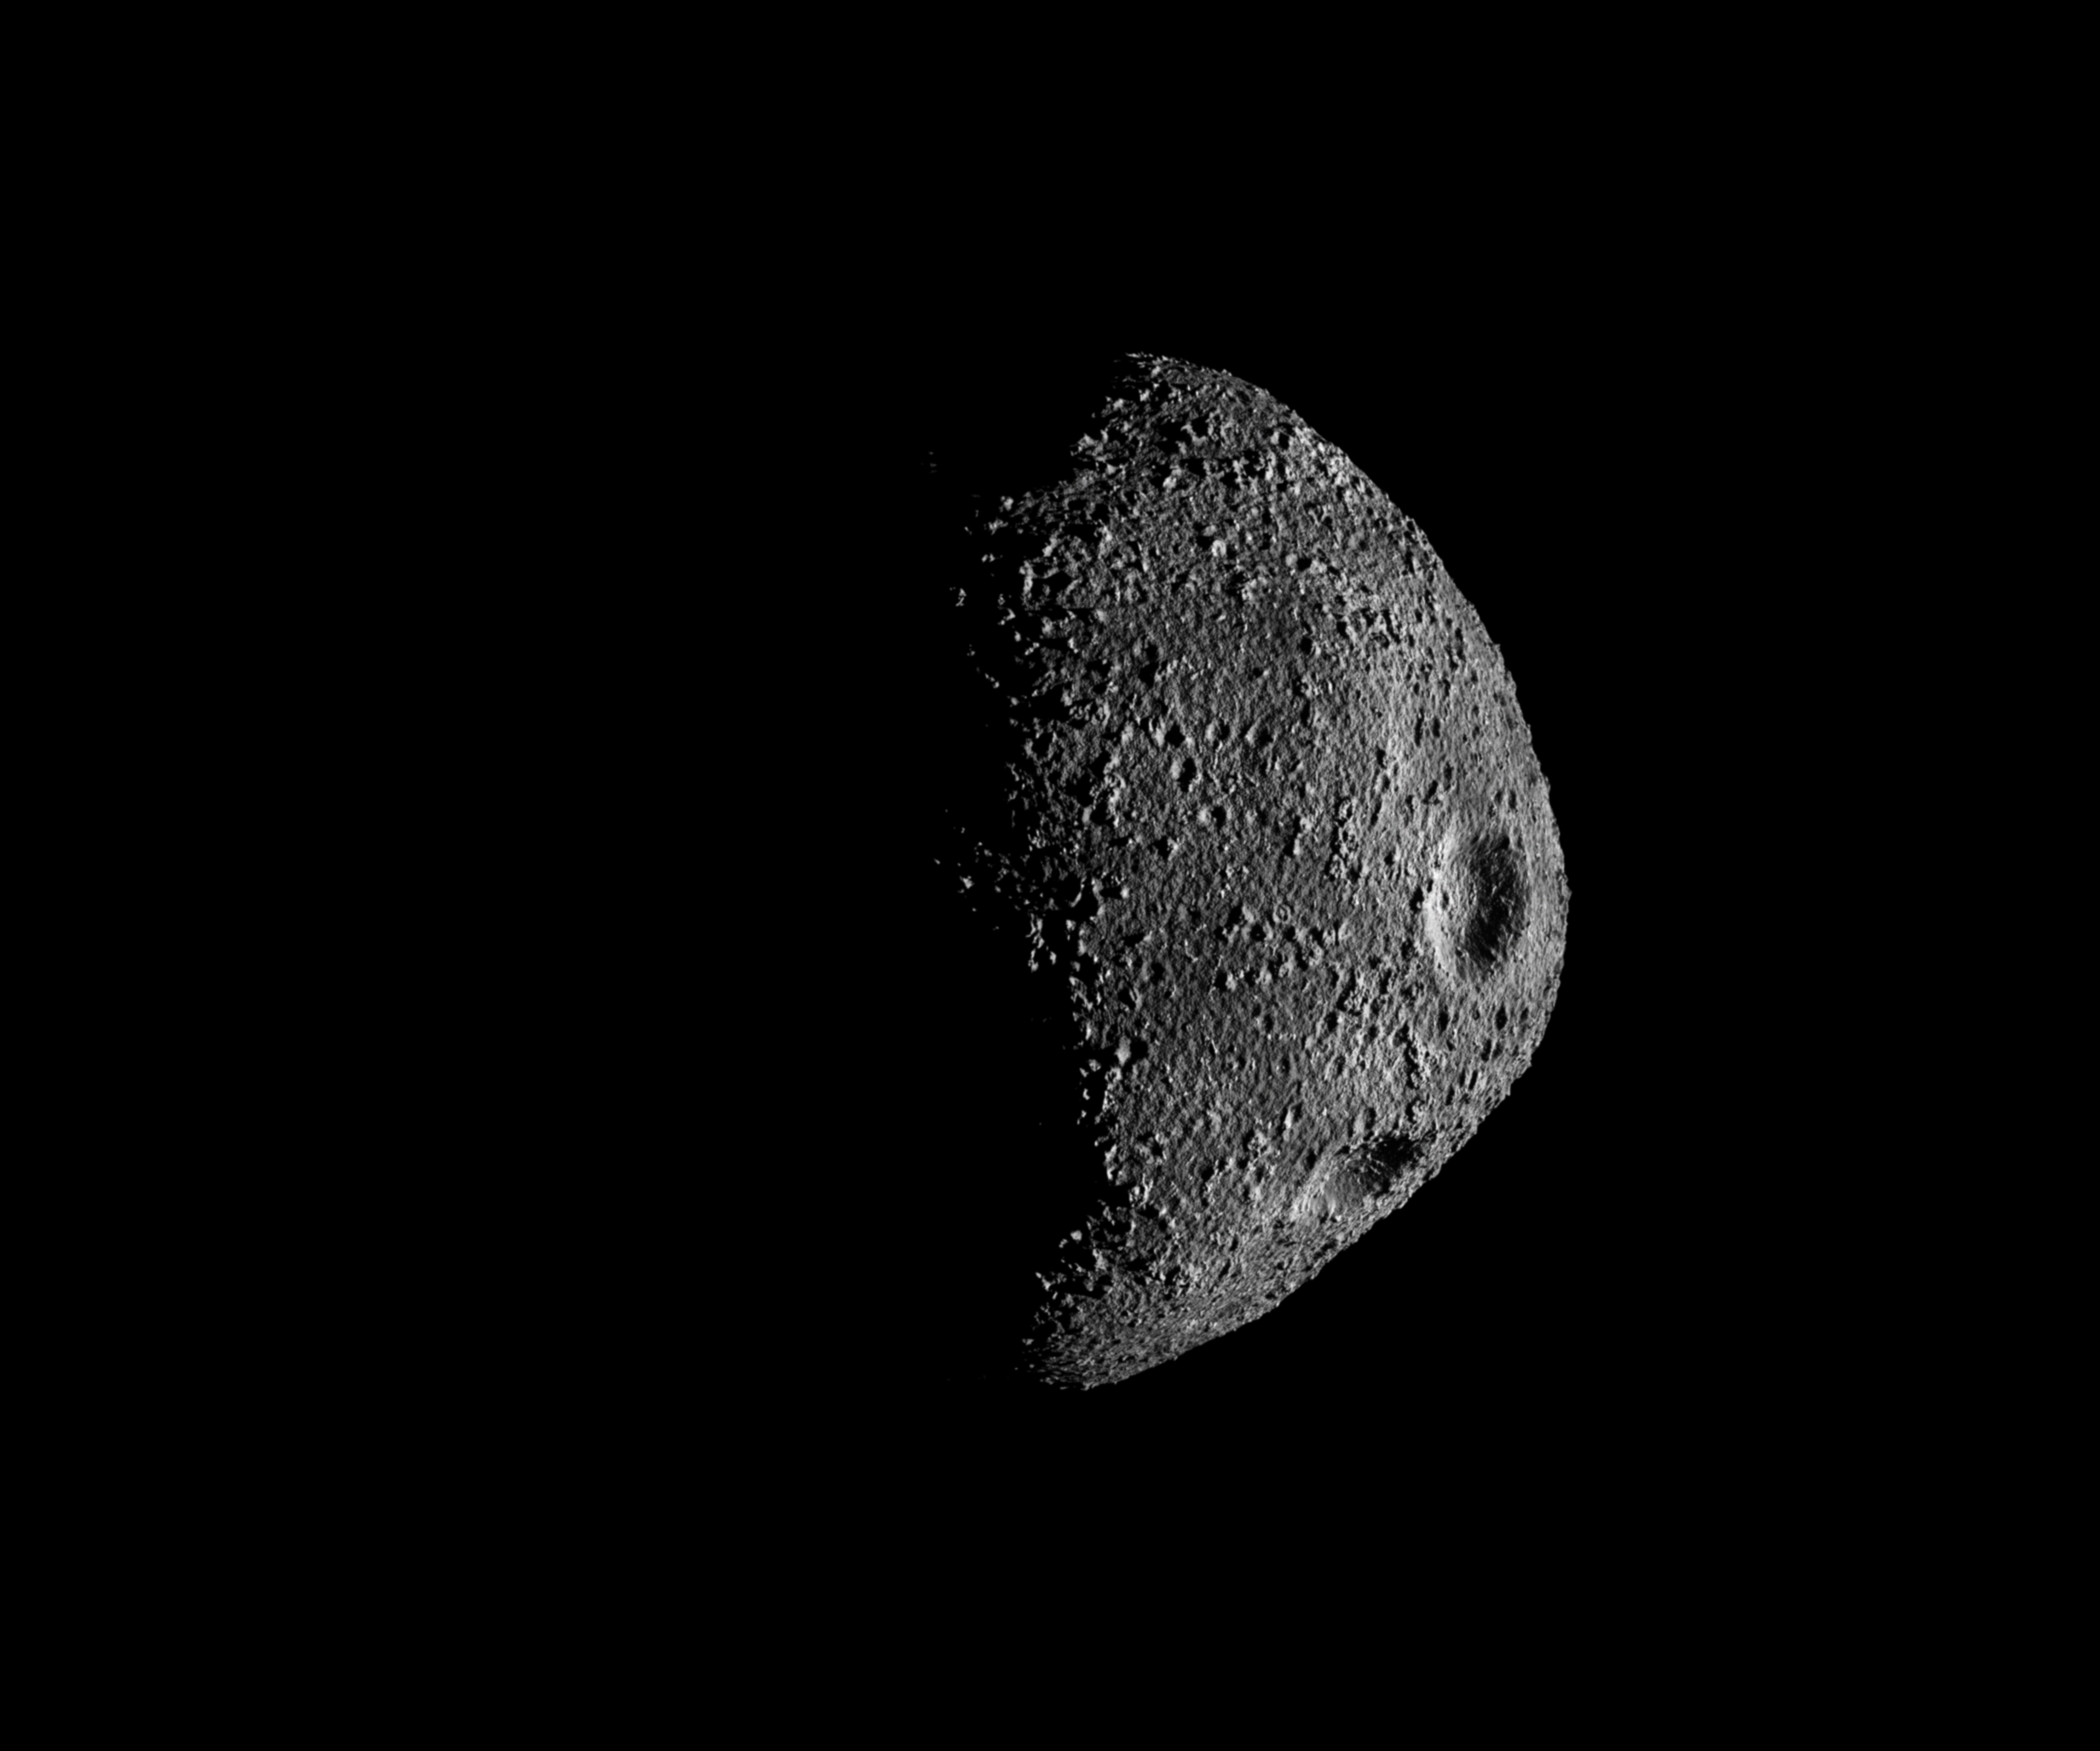
\includegraphics[width=\textwidth]{doc/thesis/0_figures/procedural_terrain/50_10_Inst_2017-08-15T115755-845000.png}
            \caption{\SI{566}{\kilo\meter}.}
            \label{fig:render_quali_comparison_1}
        \end{subfigure}
        \\
        \begin{subfigure}[b]{0.48\textwidth}
            \centering
                \includegraphics[width=\textwidth]{doc/thesis/0_figures/procedural_terrain/50_10_Inst_2017-08-15T115855-260000.png}
            \caption{\SI{106}{\kilo\meter}.}
            \label{fig:render_quali_comparison_2}
        \end{subfigure}
    \caption{Surface of a \SI{10}{\kilo\meter} \gls{sssb} at the given distances.}
    \label{fig:render_quali_comparison}
\end{figure}

\begin{figure}[htb]
    \centering
    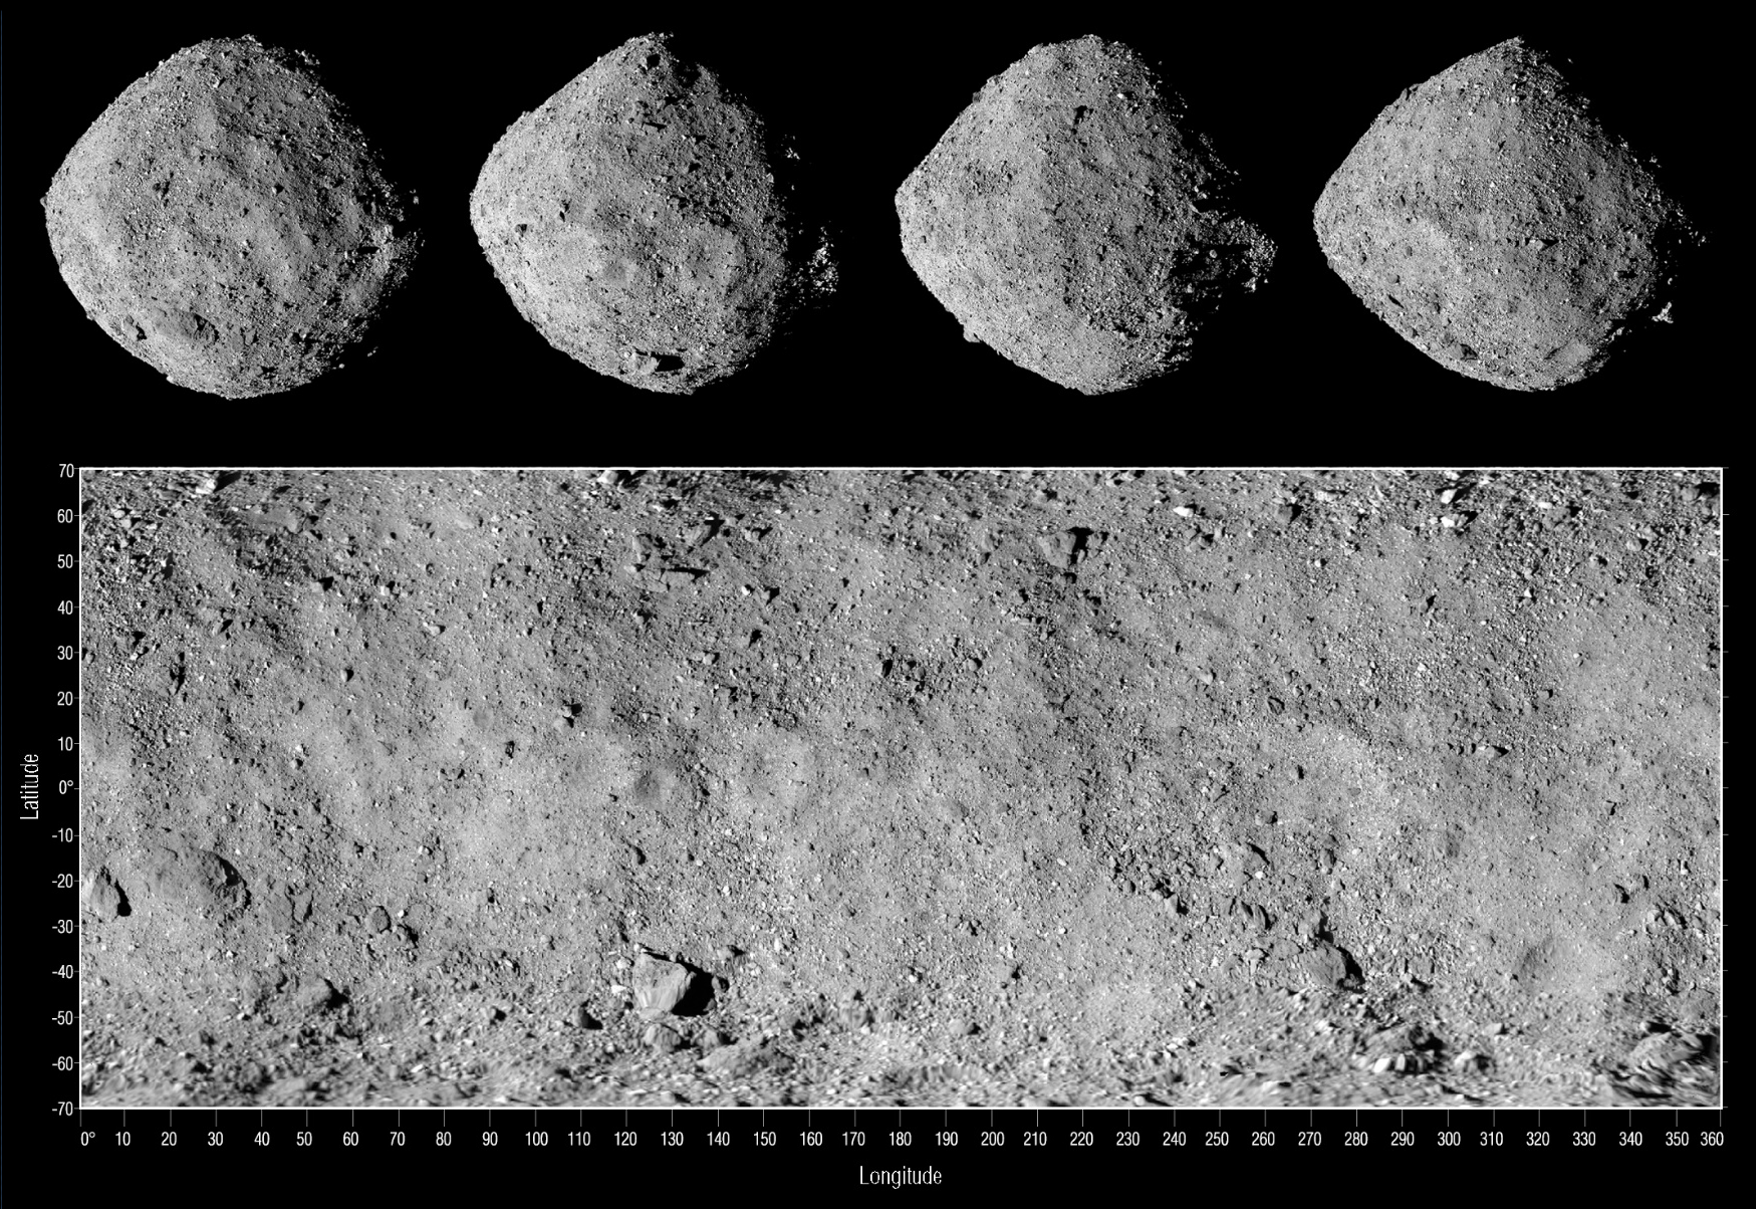
\includegraphics[width=.8\textwidth]{doc/thesis/0_figures/procedural_terrain/2963_Bennu.png}
    \caption{Four images of asteroid Bennu and a global surface mosaic. These images were taken by the PolyCam aboard the \textit{OSIRIS-REx} mission \cite{FourExploration}.}
    \label{fig:render_quali_bennu}
\end{figure}

\begin{figure}[htb]
    \centering
    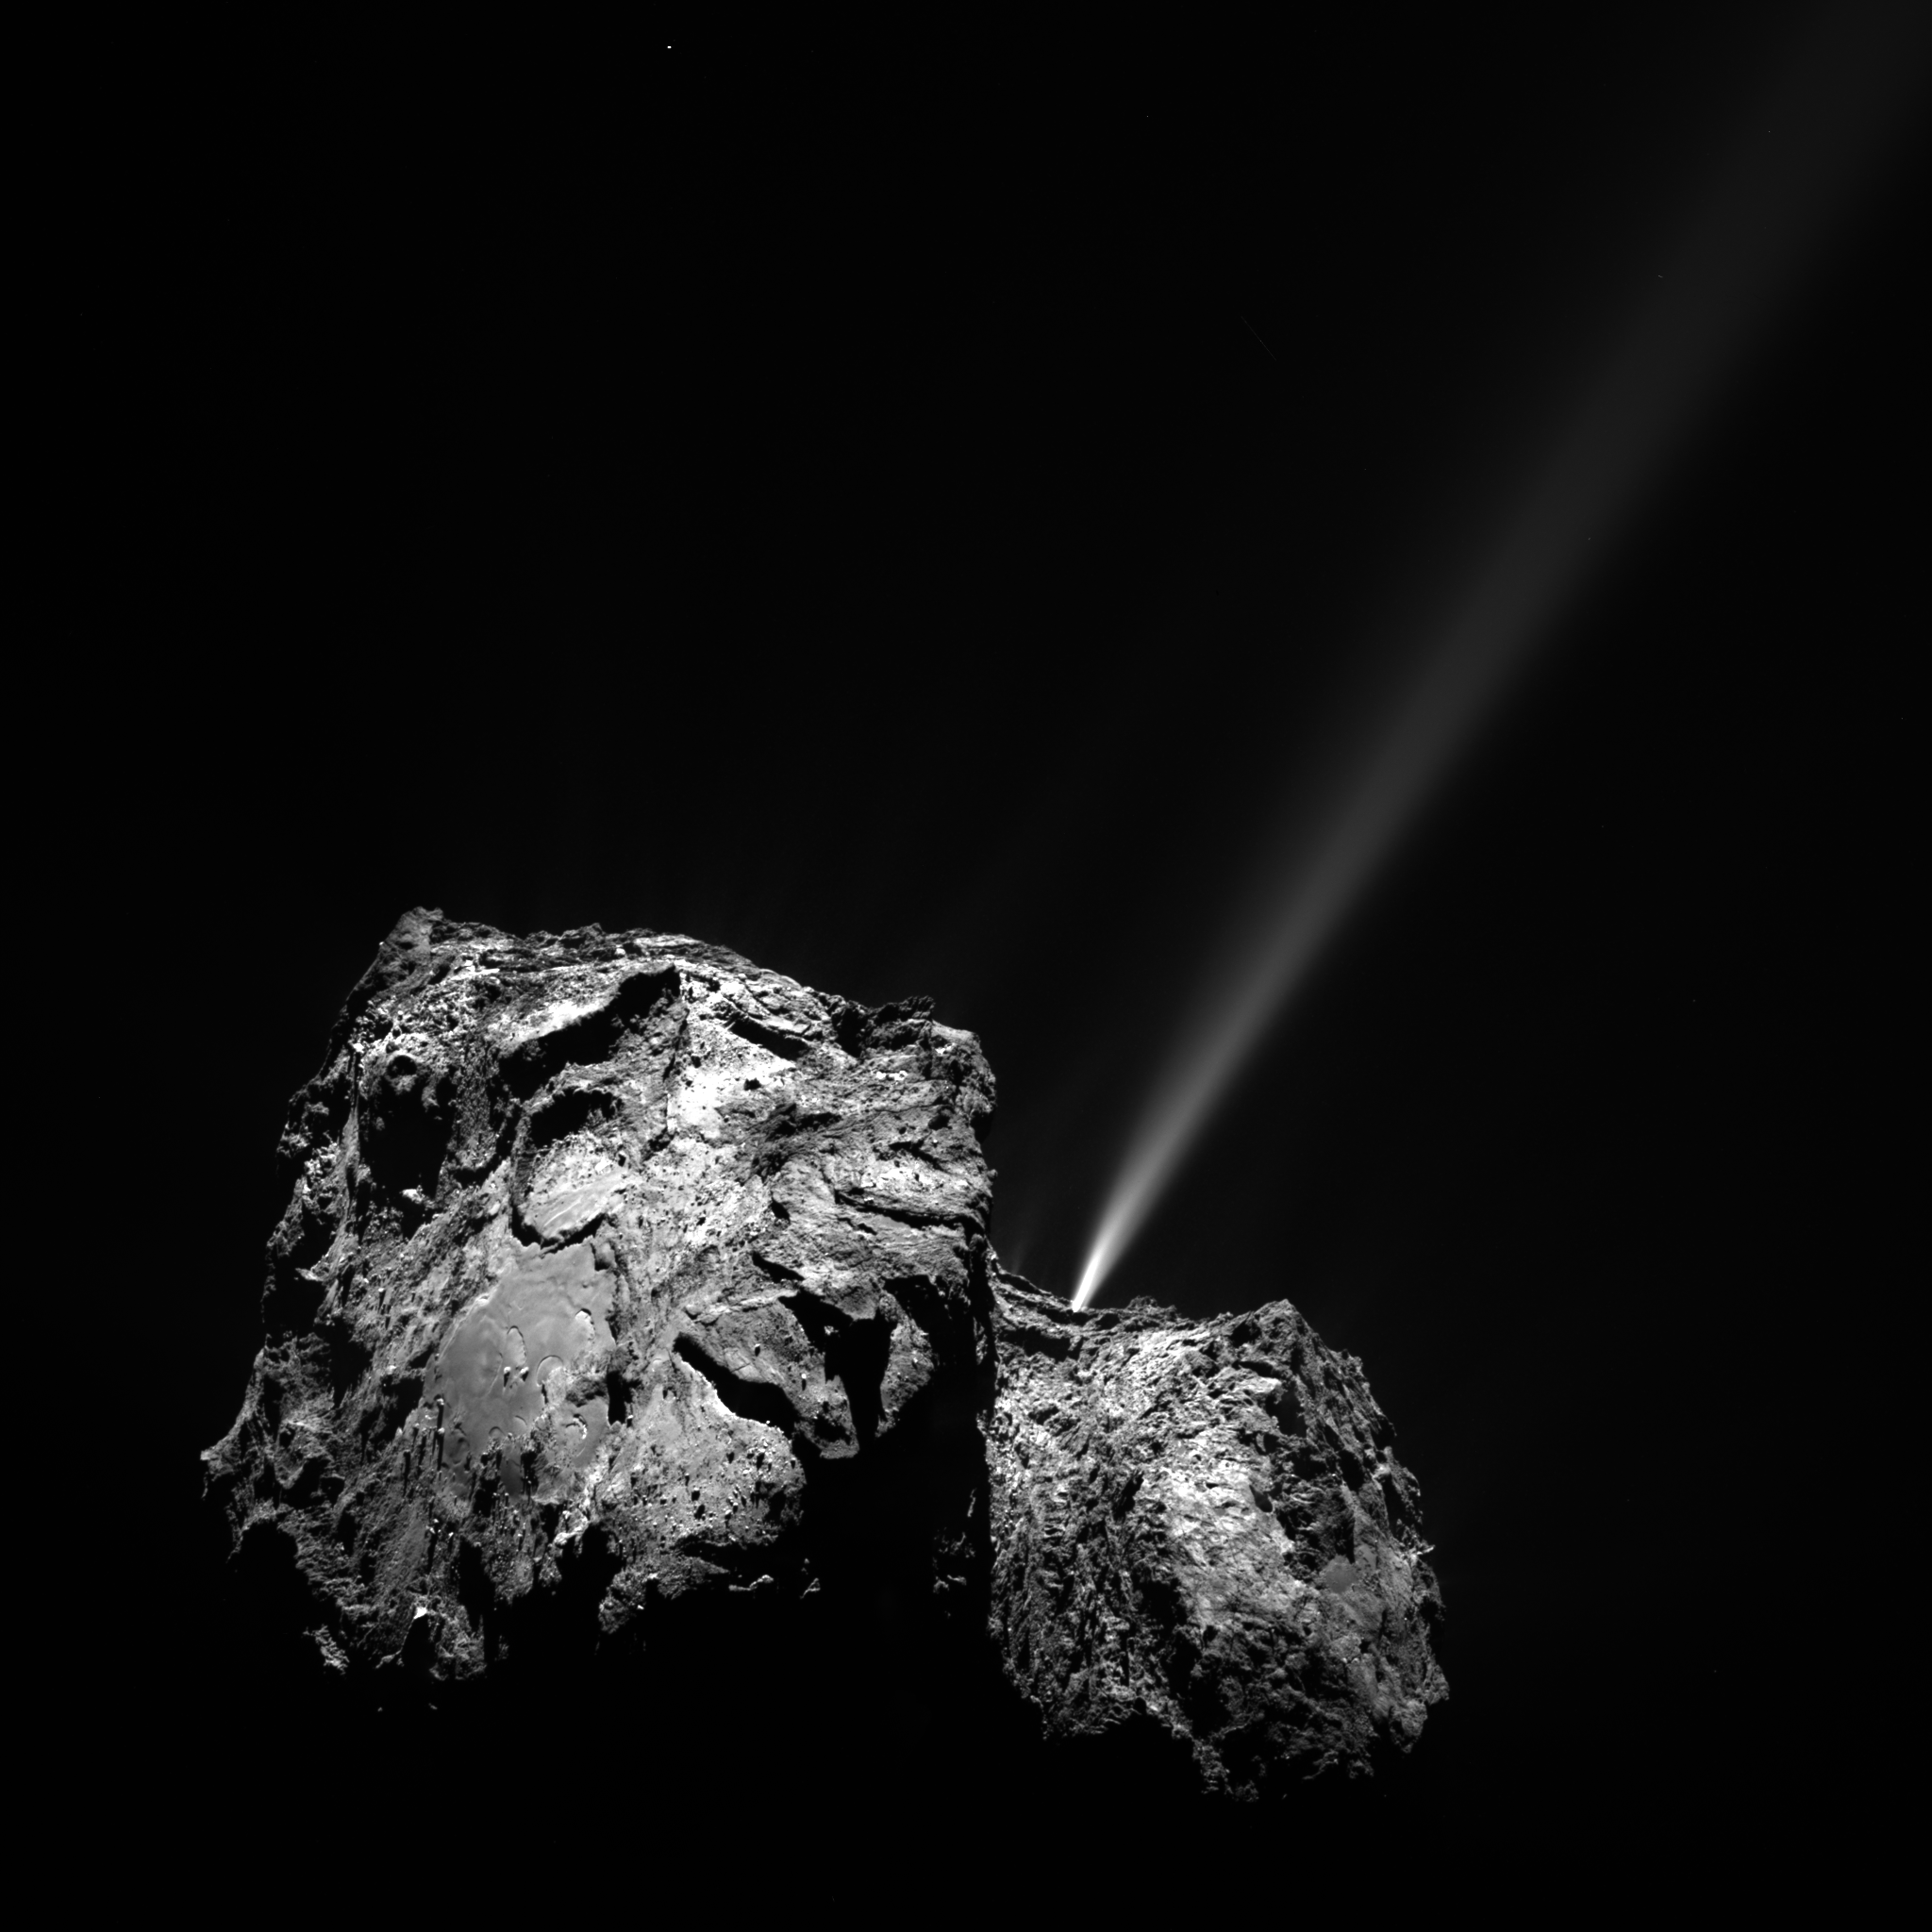
\includegraphics[width=.8\textwidth]{doc/thesis/0_figures/procedural_terrain/67P_CG.PNG}
    \caption{Representative image of comet \acrlong{67p}. This image was taken by the OSIRIS imager aboard the \textit{Rosetta} mission \cite{OSIRISArchiveb}}.
    \label{fig:render_quali_67p}
\end{figure}

\begin{figure}[htb]
    \centering
    \includegraphics[width=.8\textwidth]{doc/thesis/0_figures/procedural_terrain/Wild2.jpg}
    \caption{Collection of images of comet \acrlong{81p} taken during the \textit{Stardust} mission by its navigation camera \cite{StardustImages}.}
    \label{fig:render_quali_81p}
\end{figure}

While all images exhibit show pits, the overall appearance of the rendered images resembles the smoother pits of Bennu better than the sharper pits of \gls{67p} or \gls{81p}. The overall looks of the rendered images resemble the real images of Bennu well. The rocks and boulders present on Bennu's surface are also visible in the rendered images. When comparing the rendered images to the image of \gls{67p} or \gls{81p}, the most pronounced difference are the jets. \Gls{sispo} does not contain a gas and dust model that would produce a coma or jets and therefore these are missing in the rendered images. While the surface of both comets also feature some rocks and boulders, it is more defined by ridge-like structures. This type of feature is missing in the rendered images. Hence, the rendering output of \gls{sispo} better represents asteroids than comets.

\subsubsection{Different Distances}
Through procedural terrain generation, \gls{sispo} produces results for a large range of encounter distances. Example images with different surface distances and \gls{sssb} sizes are shown in Figure \ref{fig:img_procedural_10k}.

\begin{figure}[htb]
    \centering
        \begin{subfigure}[b]{0.75\textwidth}
            \centering
            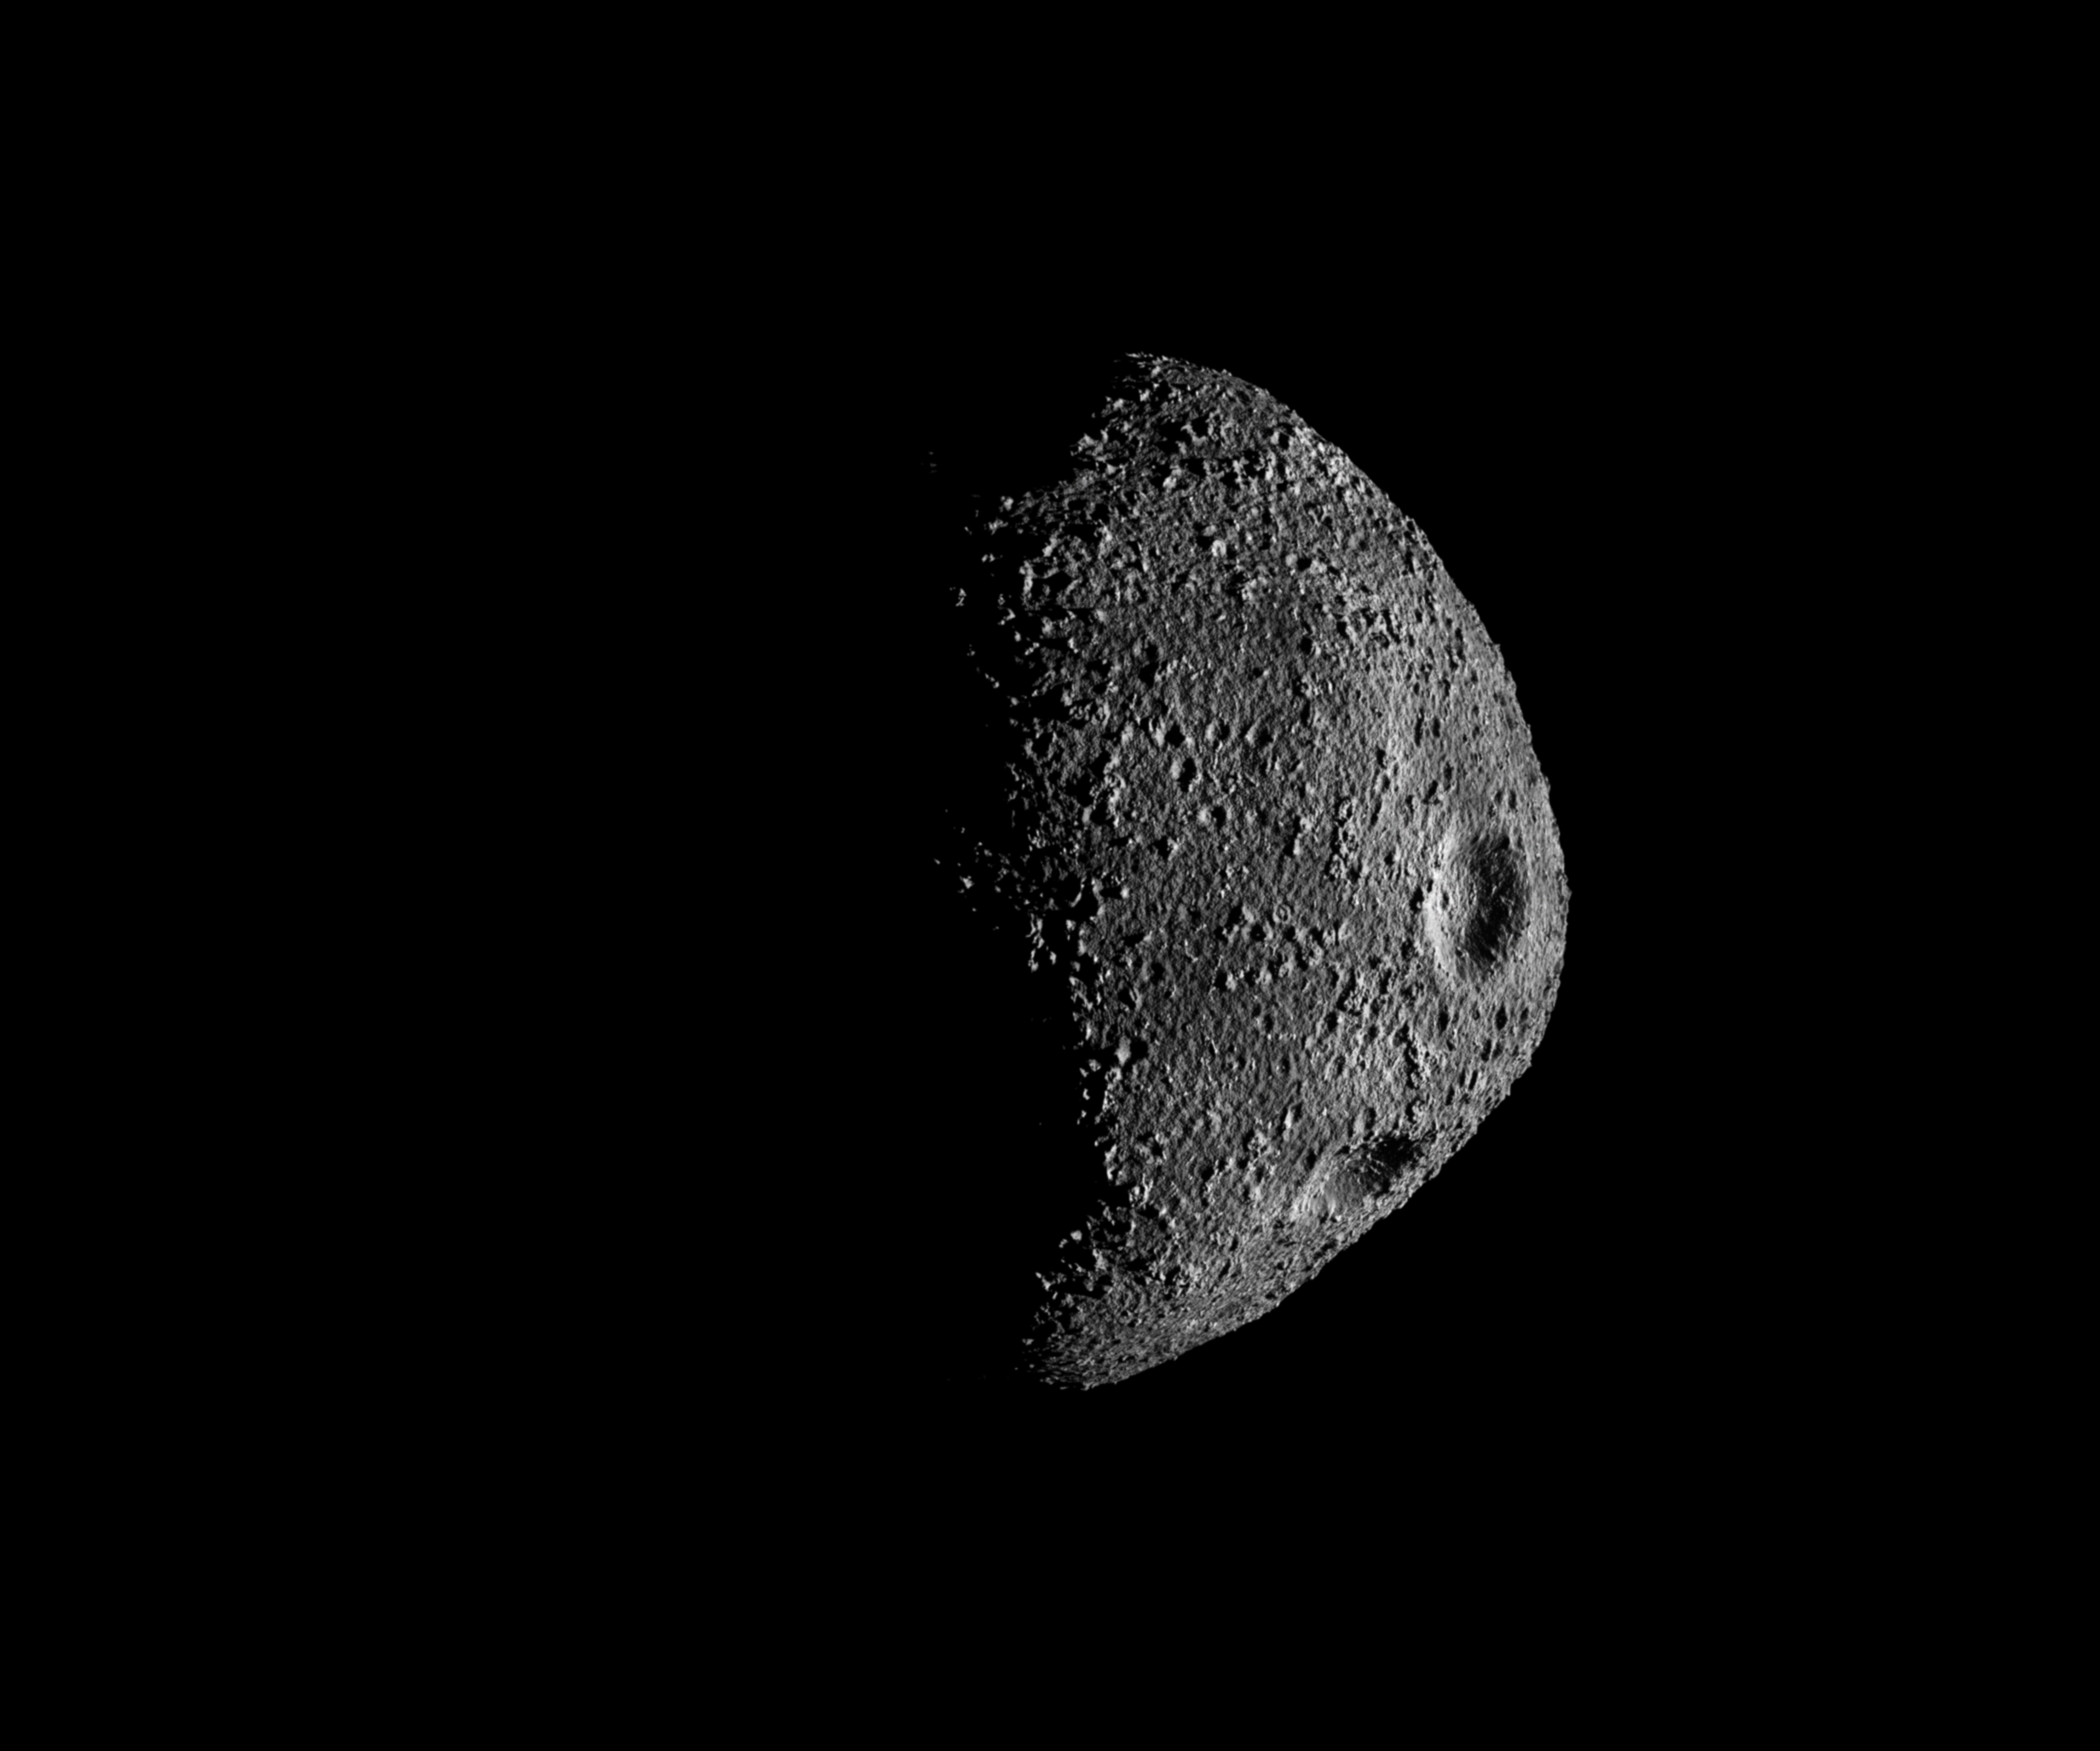
\includegraphics[width=\textwidth]{doc/thesis/0_figures/procedural_terrain/50_10_Inst_2017-08-15T115755-845000.png}
            \caption{\SI{566}{\kilo\meter}.}
            \label{fig:img_procedural_500}
        \end{subfigure}
        \\
        \begin{subfigure}[b]{0.75\textwidth}
            \centering
            \includegraphics[width=\textwidth]{doc/thesis/0_figures/procedural_terrain/50_10_Inst_2017-08-15T115855-260000.png}
            \caption{\SI{106}{\kilo\meter}.}
            \label{fig:img_procedural_100}
        \end{subfigure}
    \caption{Surface of a \SI{10}{\kilo\meter} \gls{sssb} at the given distances.}
    \label{fig:img_procedural_10k}
\end{figure}

It is visible from Figure \ref{fig:img_procedural_10k} that surface features and details do not degrade visually. Moving closer to the surface reveals more details, such as tiny bumps between larger structures which are not visible from larger distances. The visible quality of surface features is defined by the shader implementation. 

\subsubsection{Composition}
The composition process uses raw images rendered with Blender and produces photometrically calibrated images. An example set of four images consisting of two images before and after calibration is shown in Figure \ref{fig:composition_before_after}. All four images were converted to \SI{8}{\bit} images. Two effects can be seen. First, the original images differ in there overall brightness. This difference is removed by the calibration. Secondly, images become brighter by the calibration process. 

\begin{figure}[htb]
    \centering
        \begin{subfigure}[b]{0.48\textwidth}
            \centering
                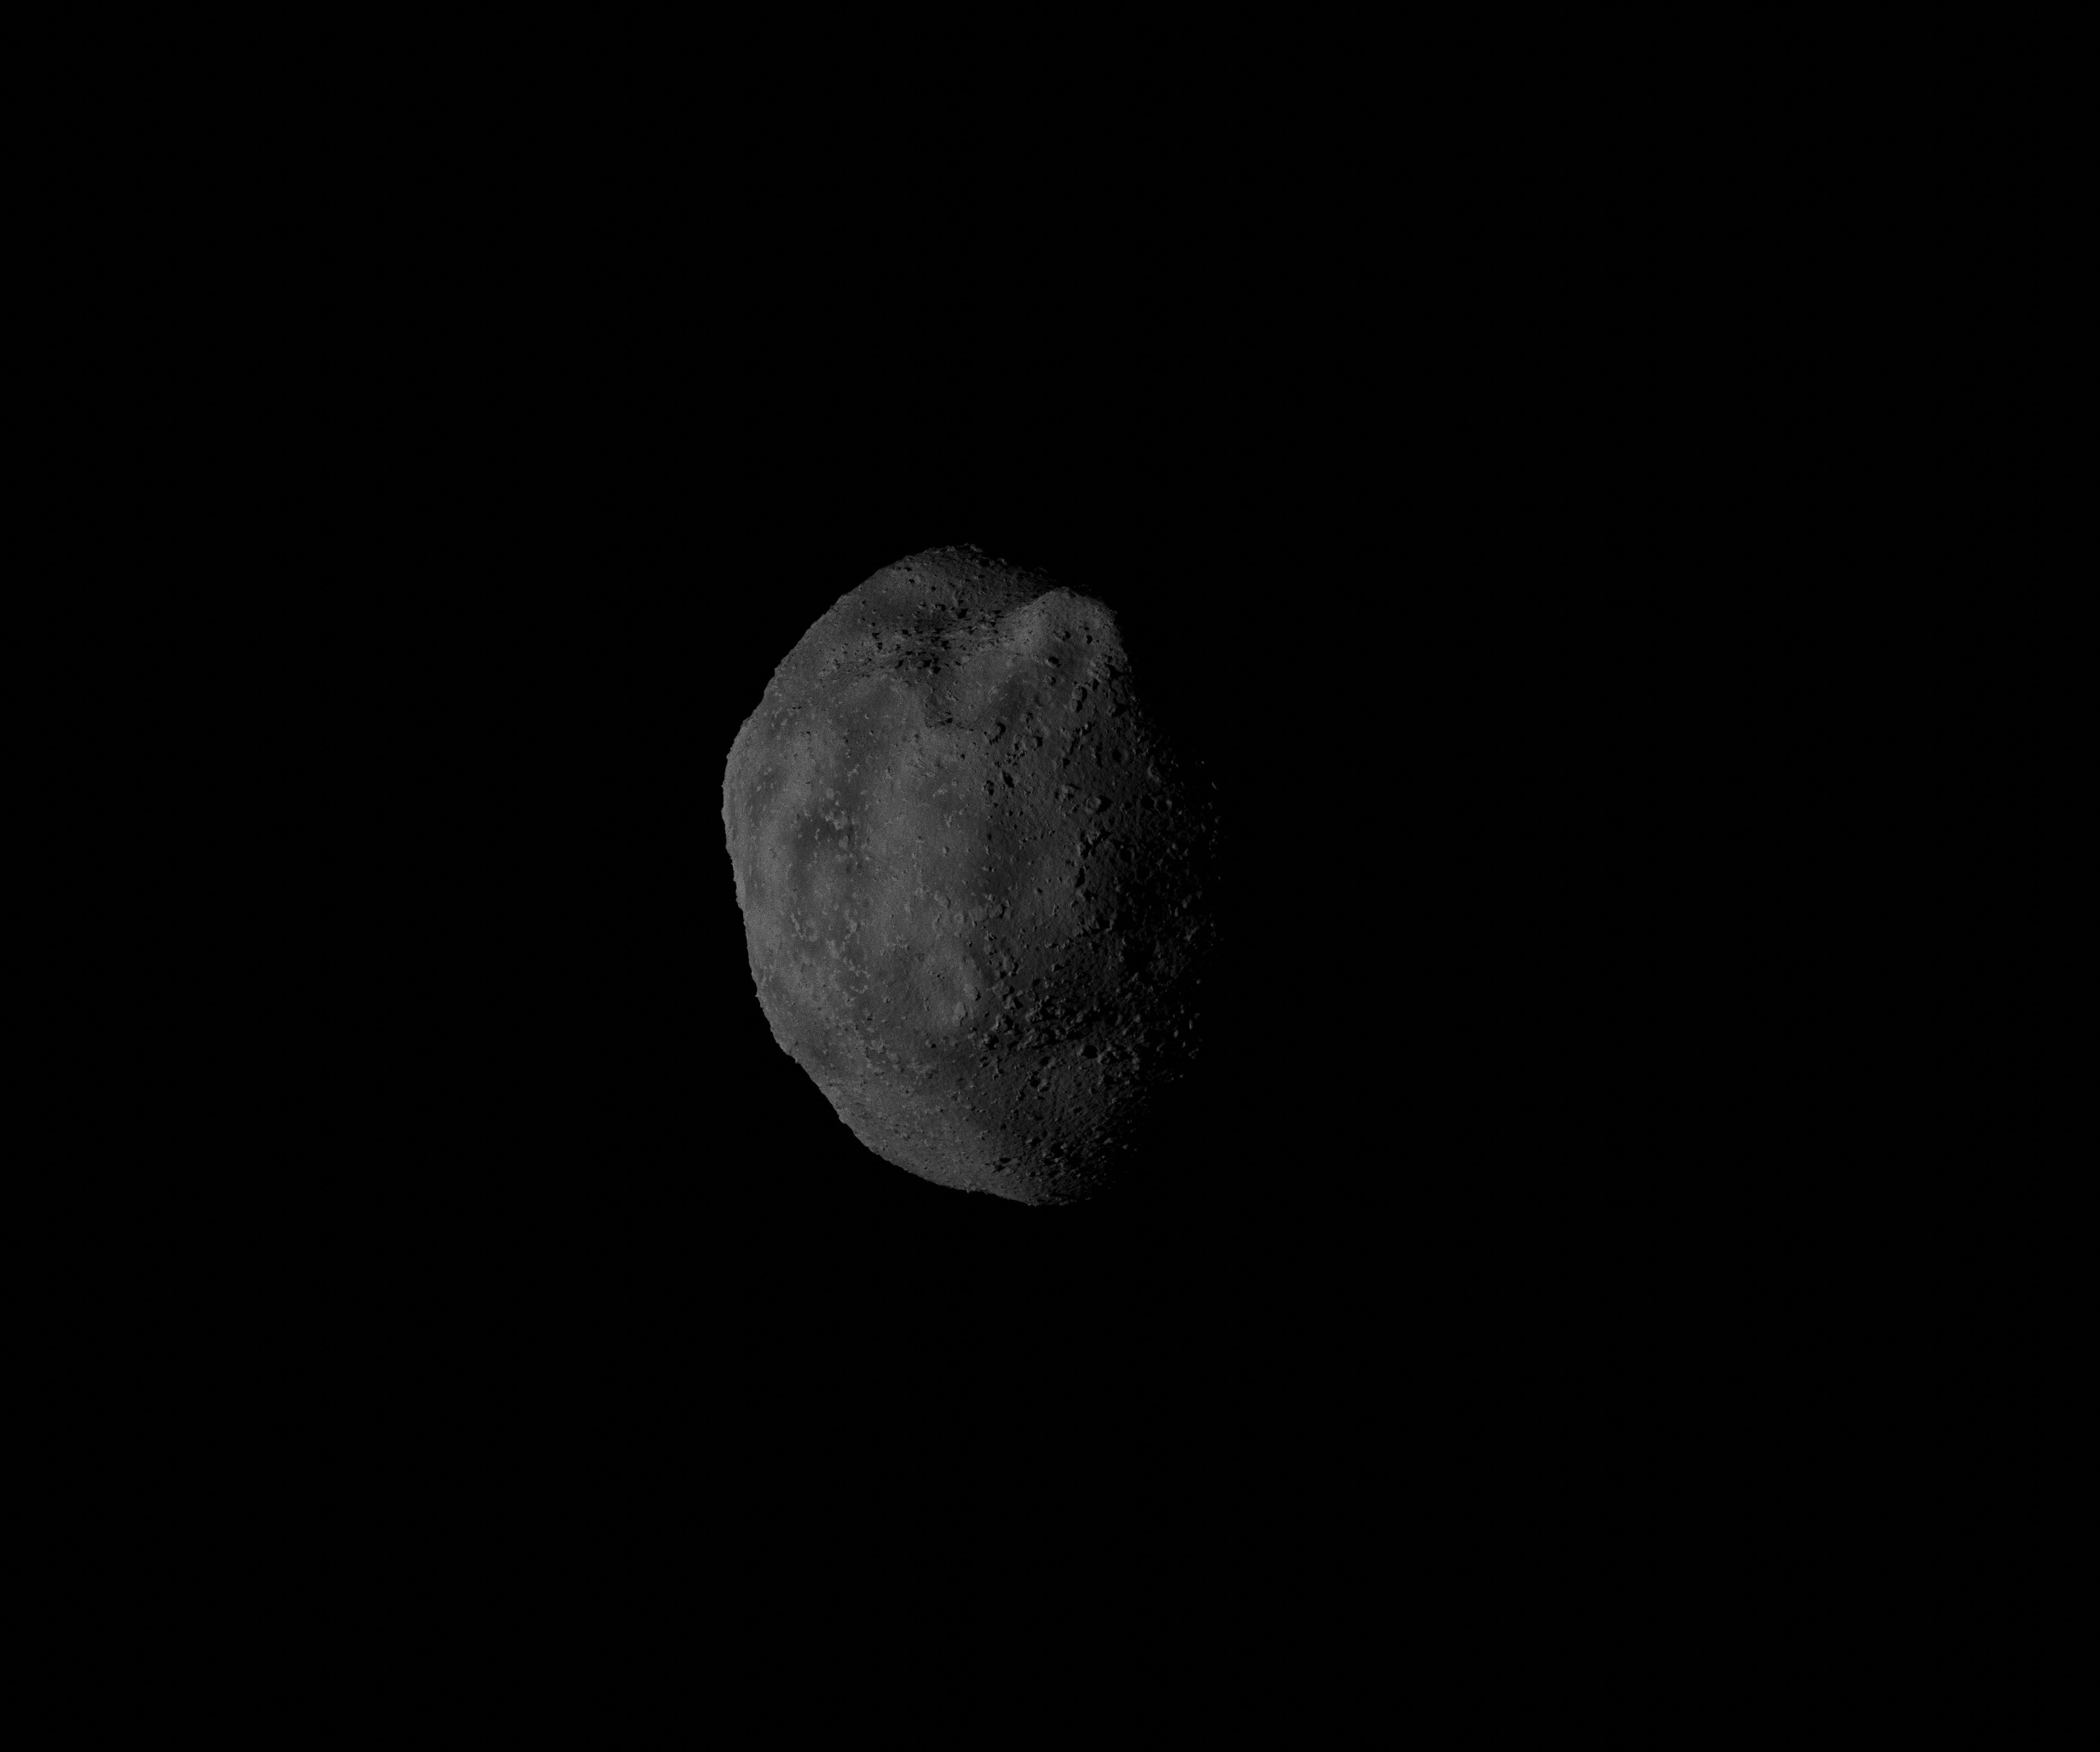
\includegraphics[width=\textwidth]{doc/thesis/0_figures/rendering_lighting/SssbOnly_2017-08-15T115858-281000.jpg}
                \caption{Image 1 before calibration.}
                \label{fig:composition_before_1}
        \end{subfigure}
        \begin{subfigure}[b]{0.48\textwidth}
            \centering
                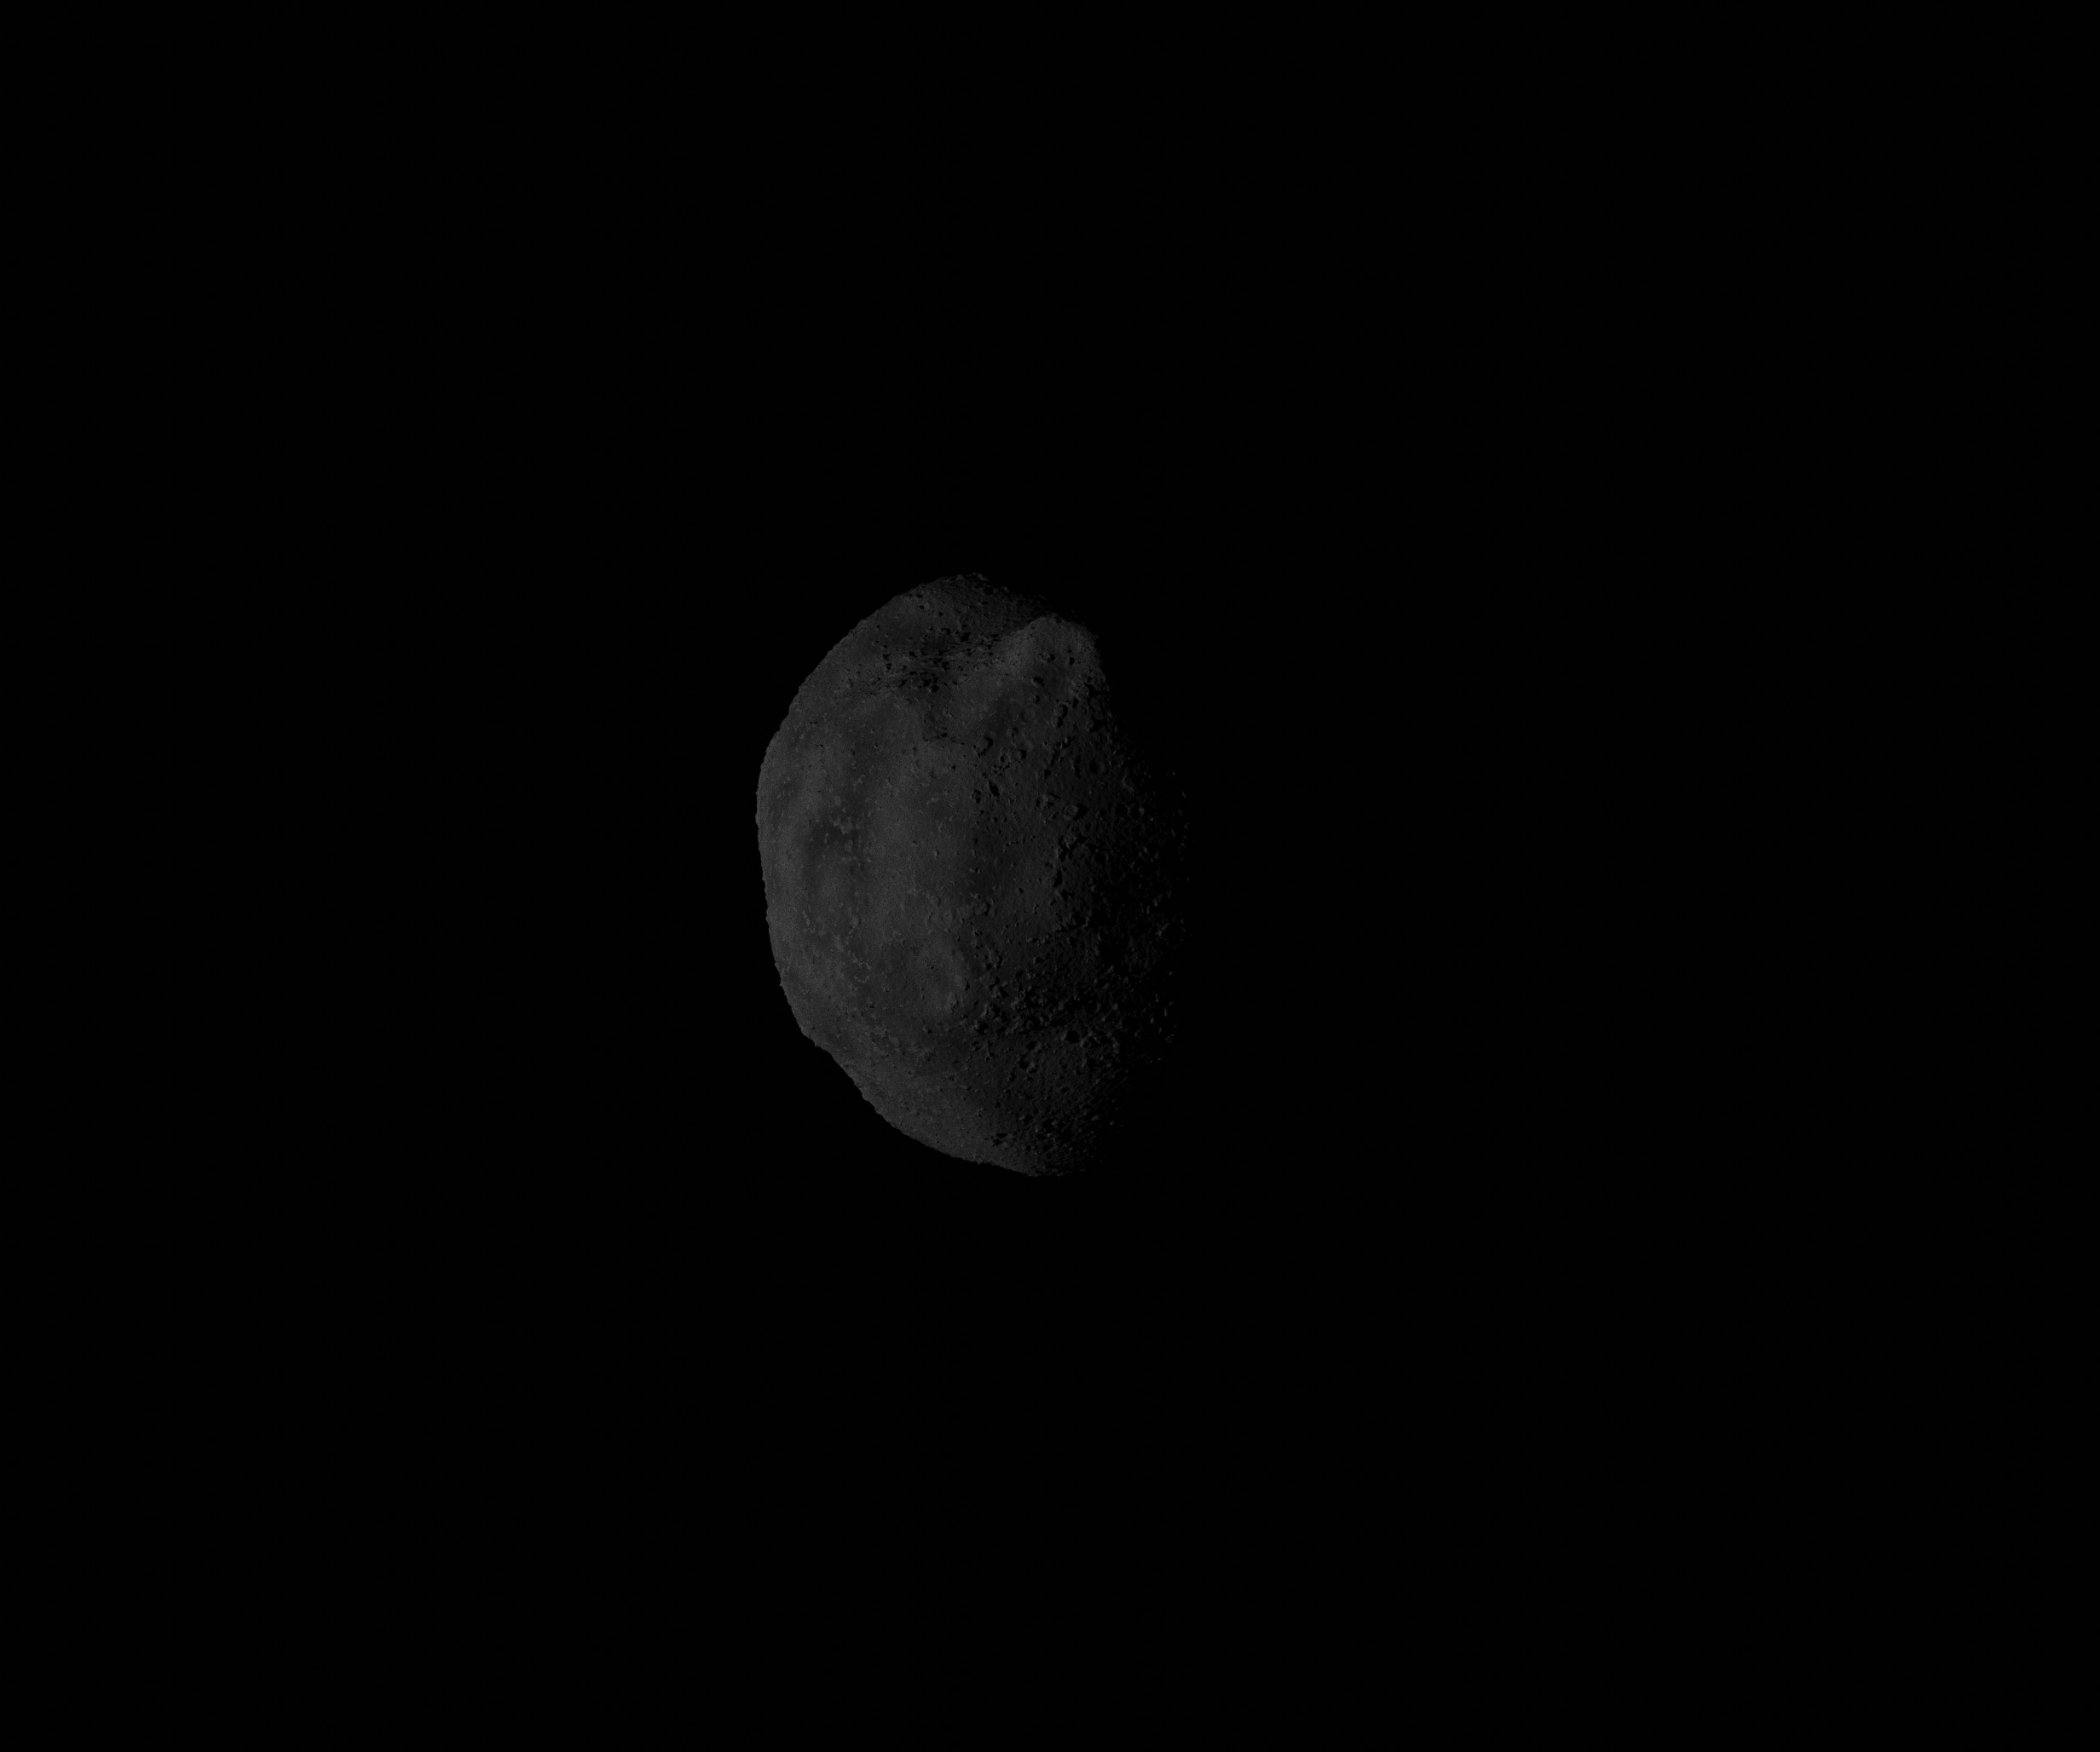
\includegraphics[width=\textwidth]{doc/thesis/0_figures/rendering_lighting/SssbOnly_2017-08-15T115859-288000.jpg}
                \caption{Image 2 before calibration.}
                \label{fig:composition_before_2}
        \end{subfigure}
        \\
        \begin{subfigure}[b]{0.48\textwidth}
            \centering
                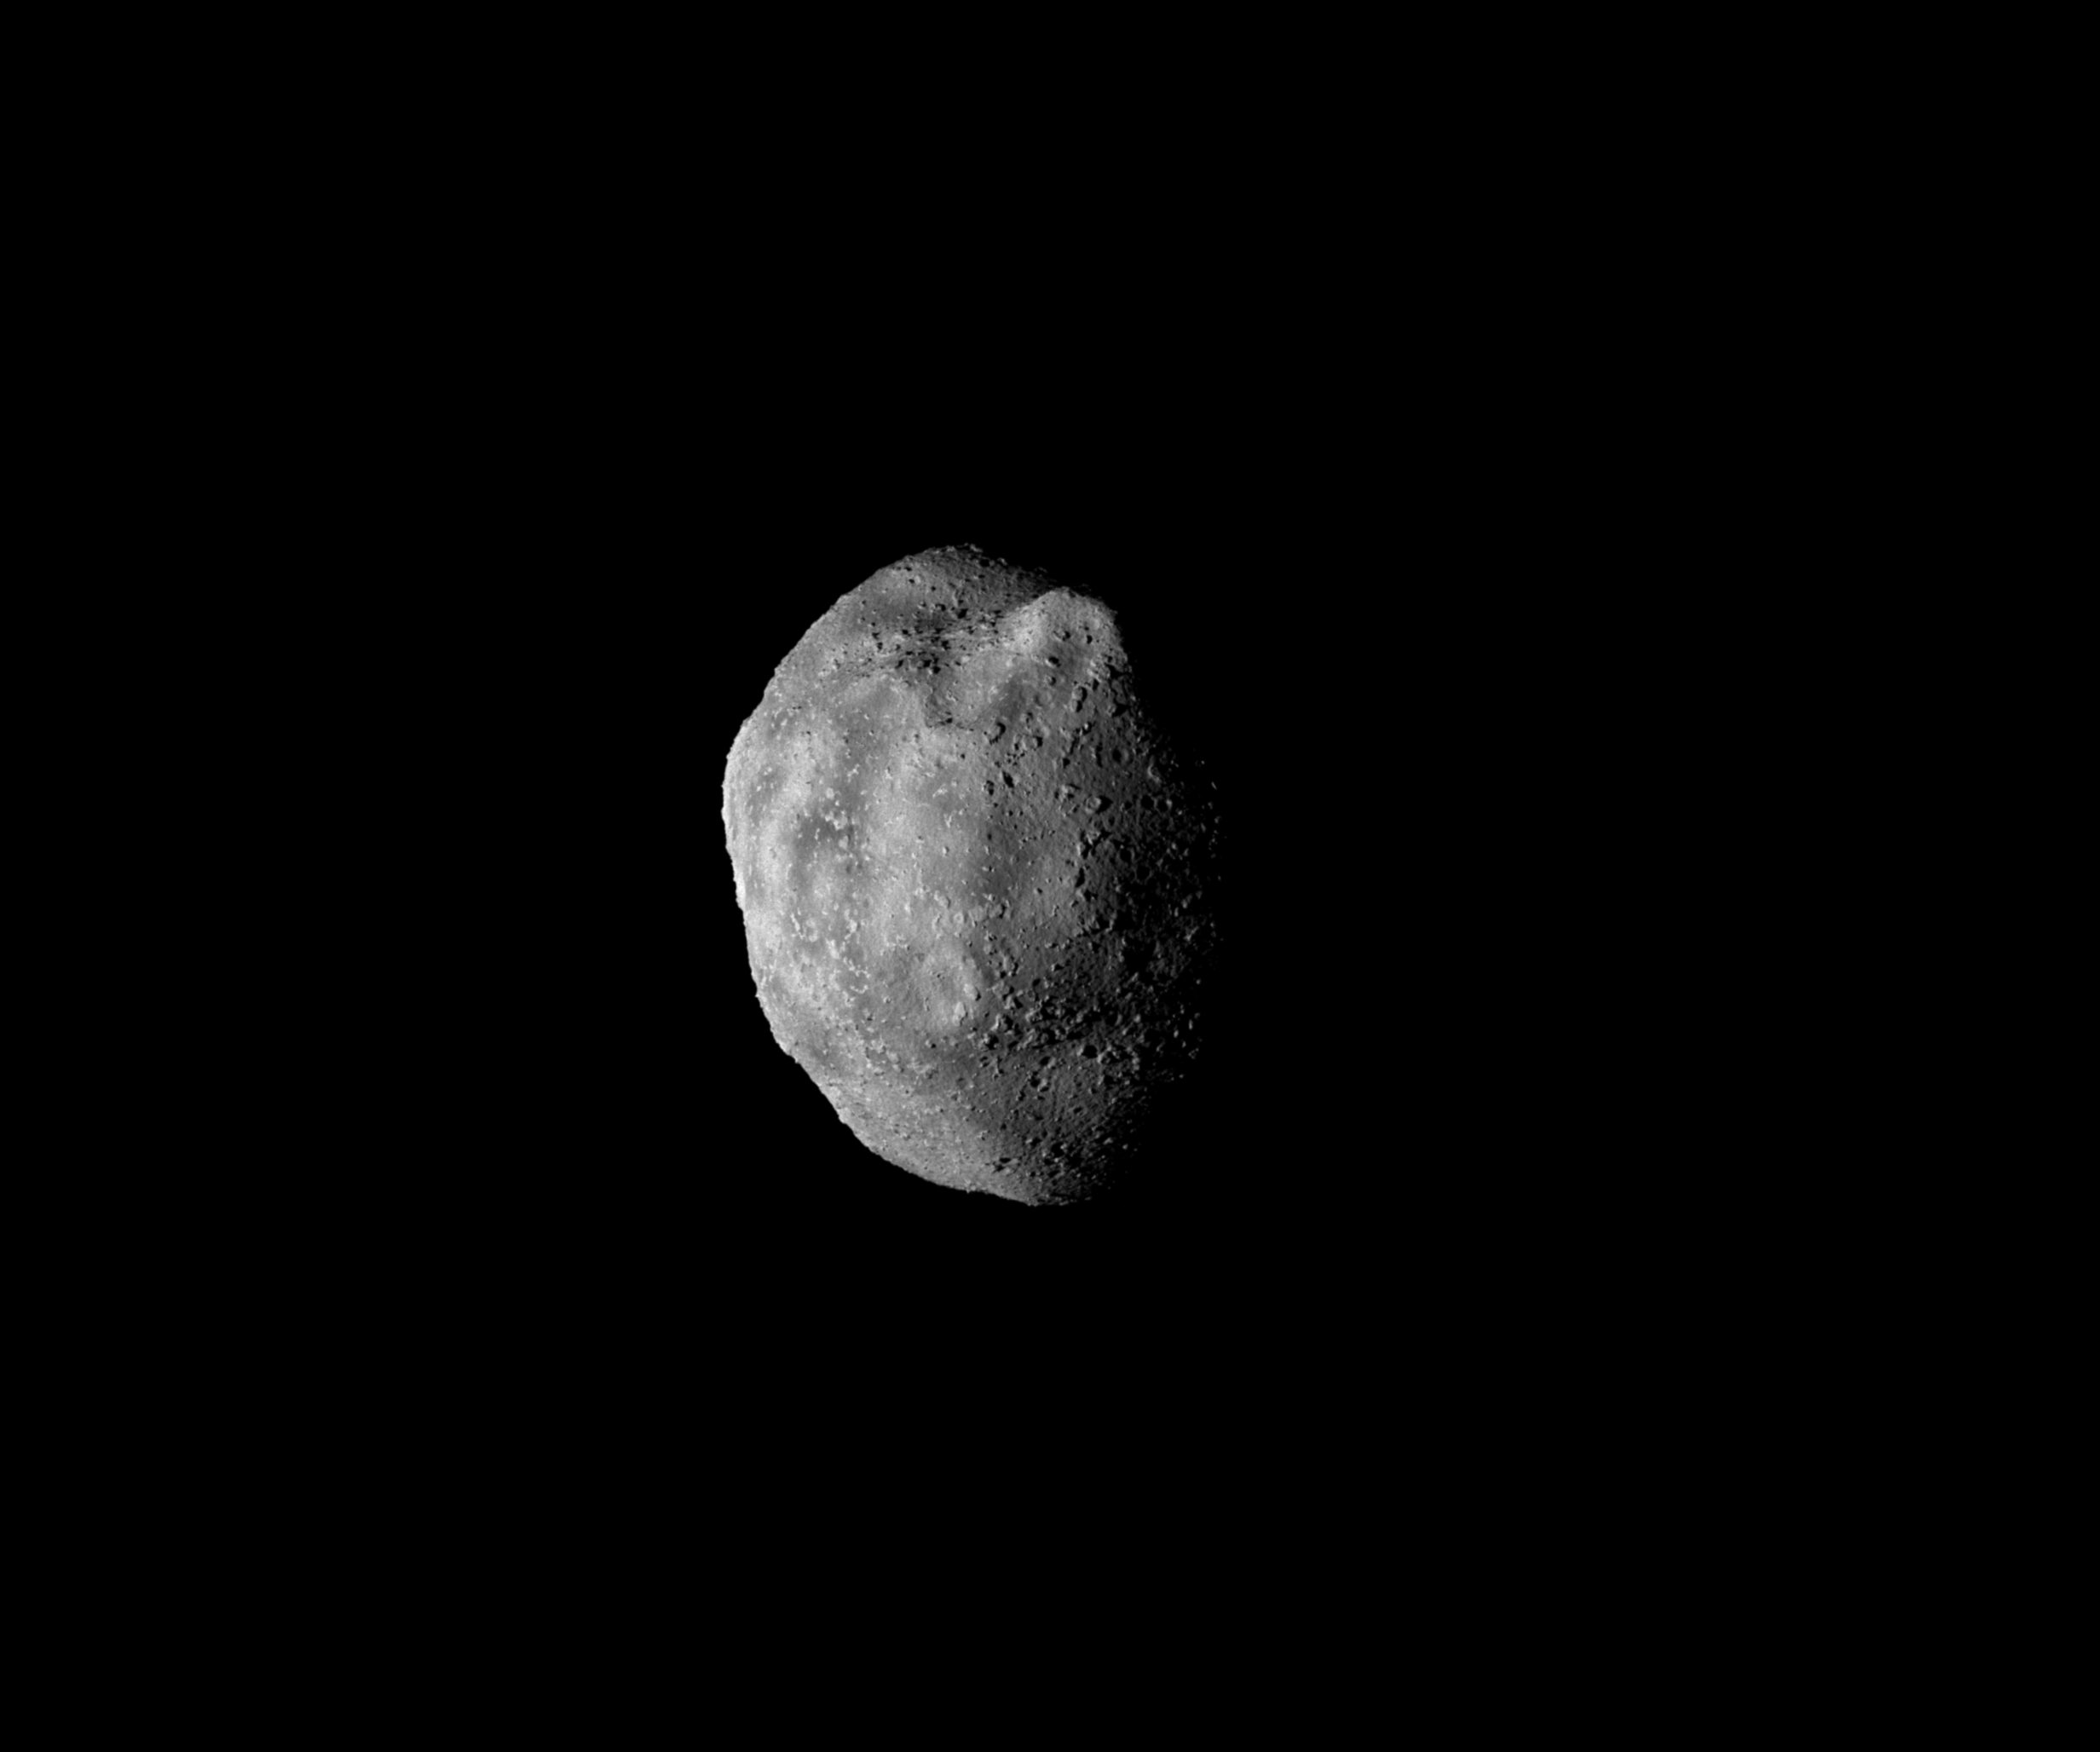
\includegraphics[width=\textwidth]{doc/thesis/0_figures/rendering_lighting/Inst_2017-08-15T115858-281000.png}
                \caption{Image 1 after calibration.}
                \label{fig:composition_after_1}
        \end{subfigure}
        \begin{subfigure}[b]{0.48\textwidth}
            \centering
                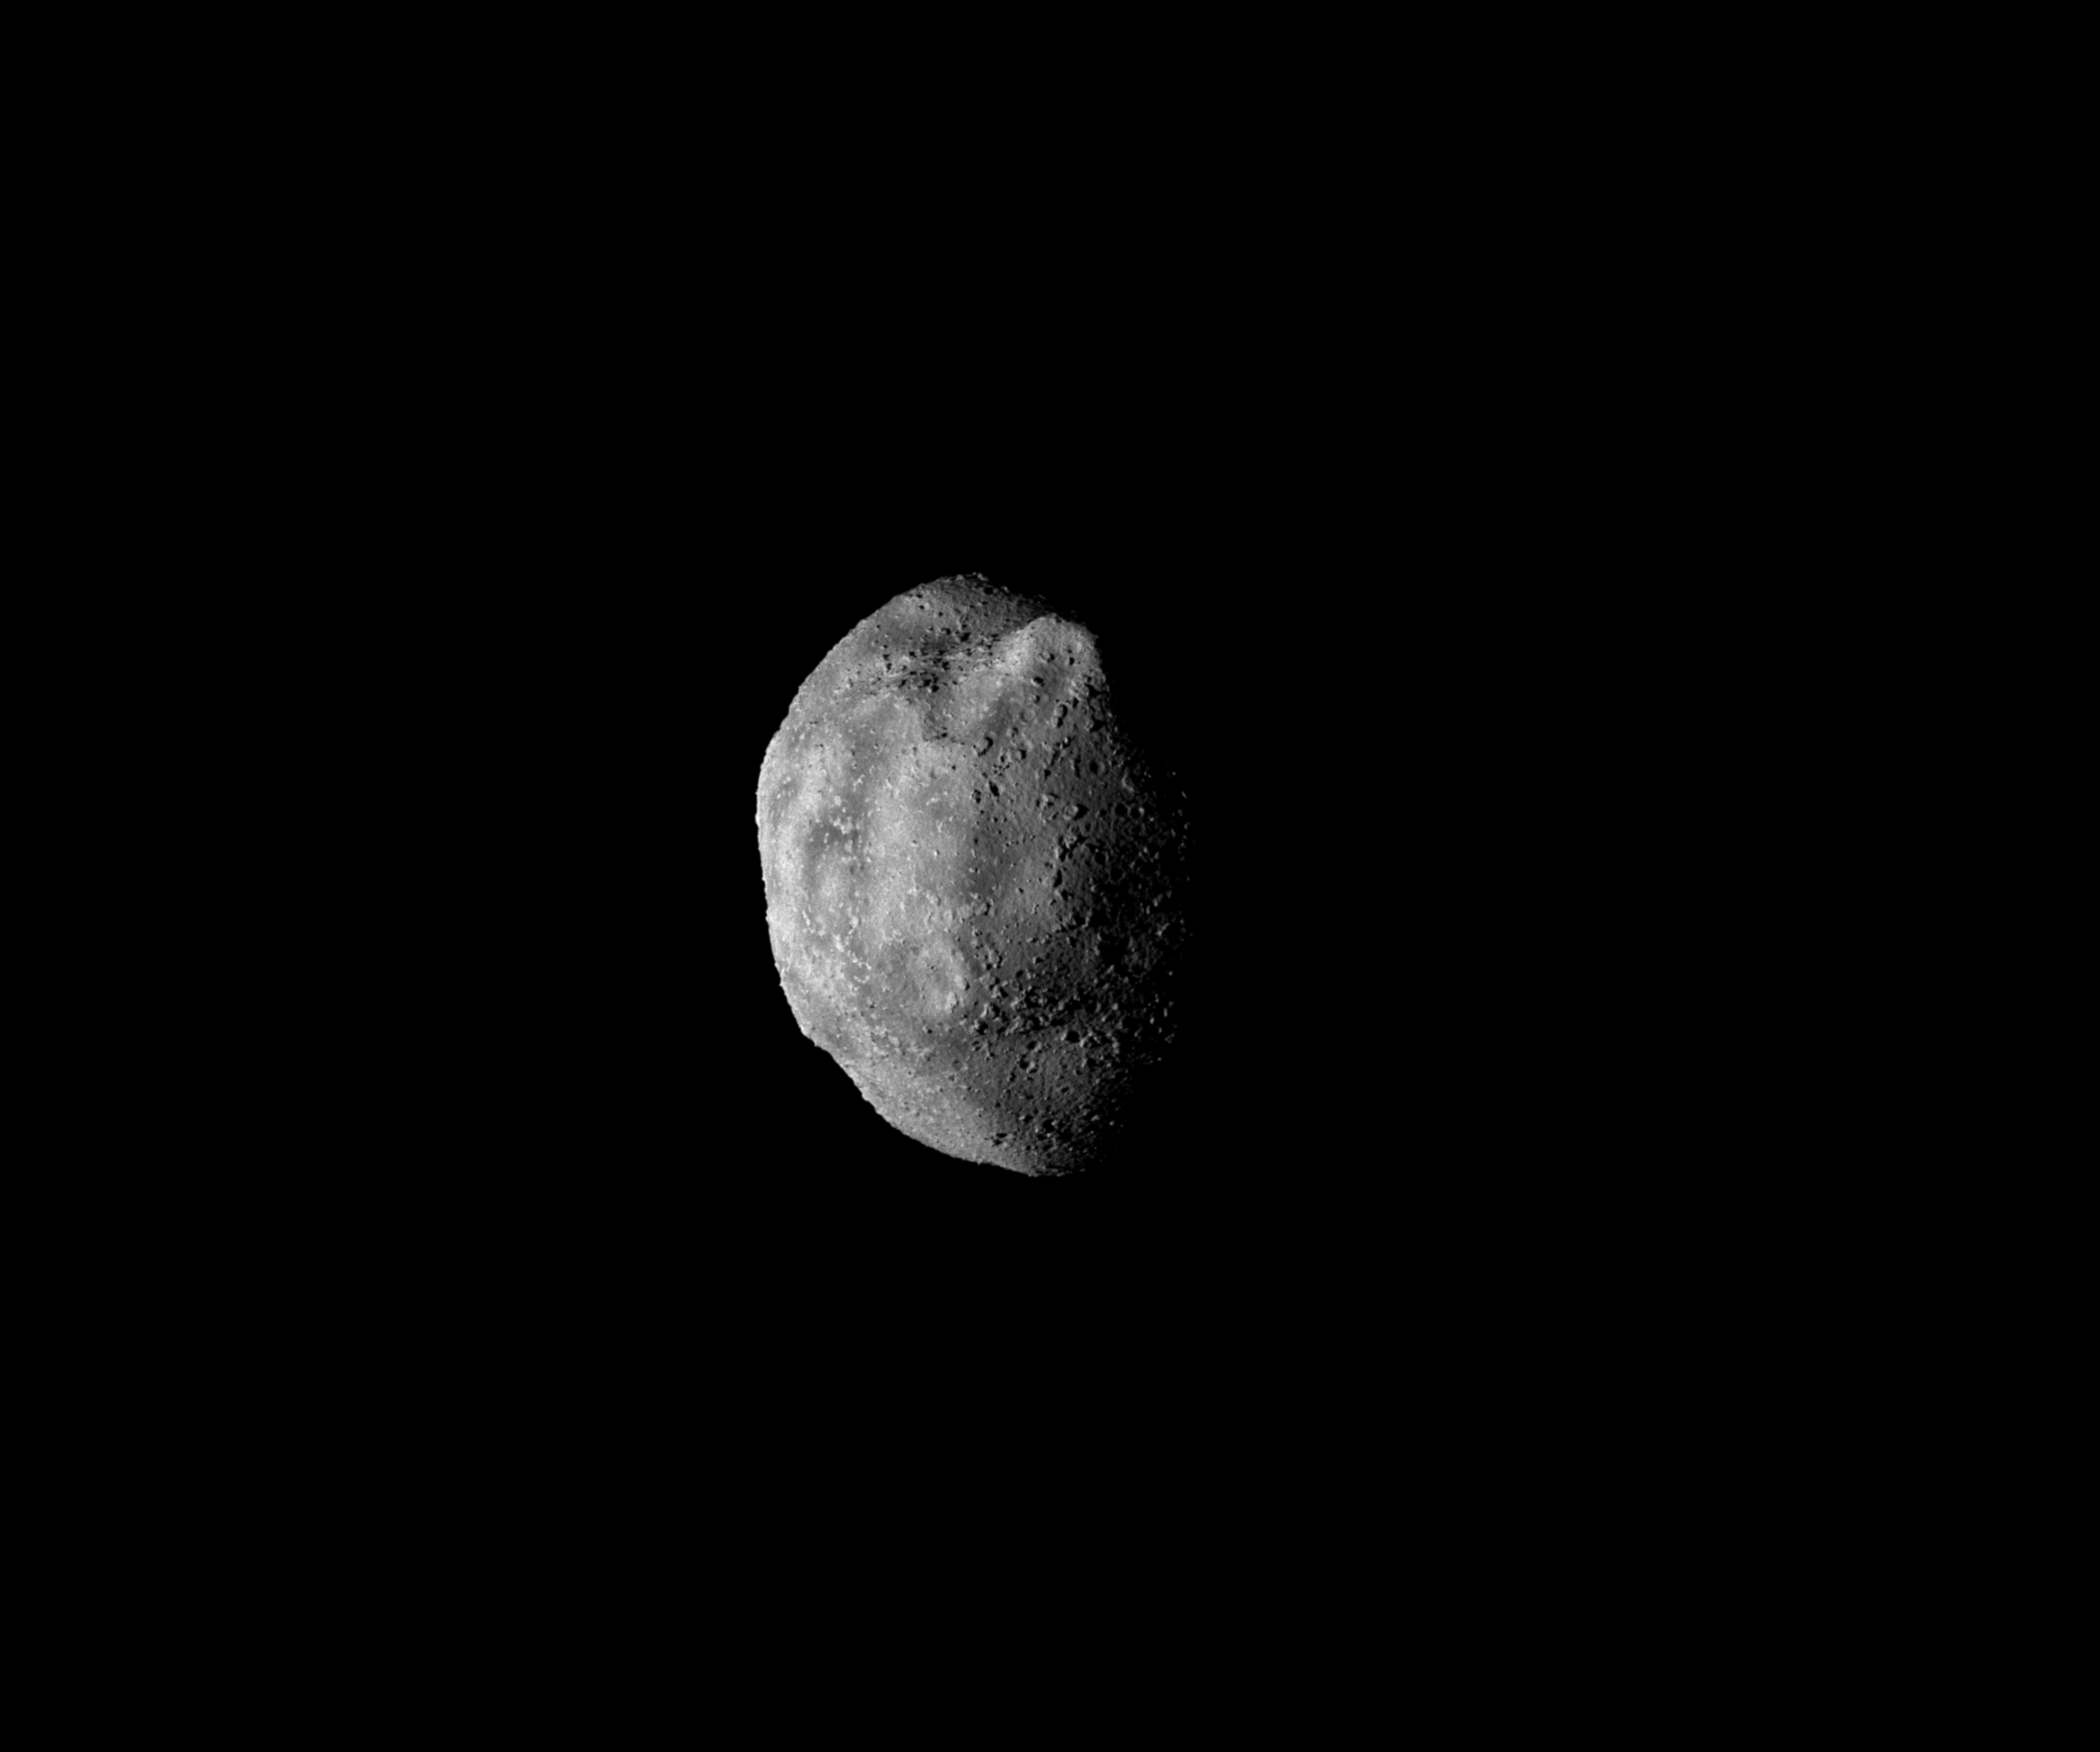
\includegraphics[width=\textwidth]{doc/thesis/0_figures/rendering_lighting/Inst_2017-08-15T115859-288000.png}
                \caption{Image 2 after calibration.}
                \label{fig:composition_after_2}
        \end{subfigure}
        \caption{Two images of a flyby, image 2 is one second after image 1, before and after the composition process. The nucleus is much brighter than background stars thus no stars visible in these images after calibration.}
        \label{fig:composition_before_after}
\end{figure}



\subsubsection{Rendering Problems}
Rendering a fly-by scenario with a \SI{10}{\kilo\meter} \gls{sssb} created artefacts in the images. Figure \ref{fig:render_artefacts} shows renders from flybys with different closest distances from the nucleus. All three images are the raw output from rendering, before composition. The images show a darker patch across the \gls{sssb} with sharp brightness transitions. Moreover, the stripe is at the same location across the \gls{sssb} in all three images. This type of artefact does not appear for other \gls{sssb} sizes. The most likely explanation are errors while scaling the nucleus from the original \SI{1}{\kilo\meter} to the \SI{10}{\kilo\meter} model.
\begin{figure}[htb]
    \centering
        \begin{subfigure}[b]{0.32\textwidth}
            \centering
            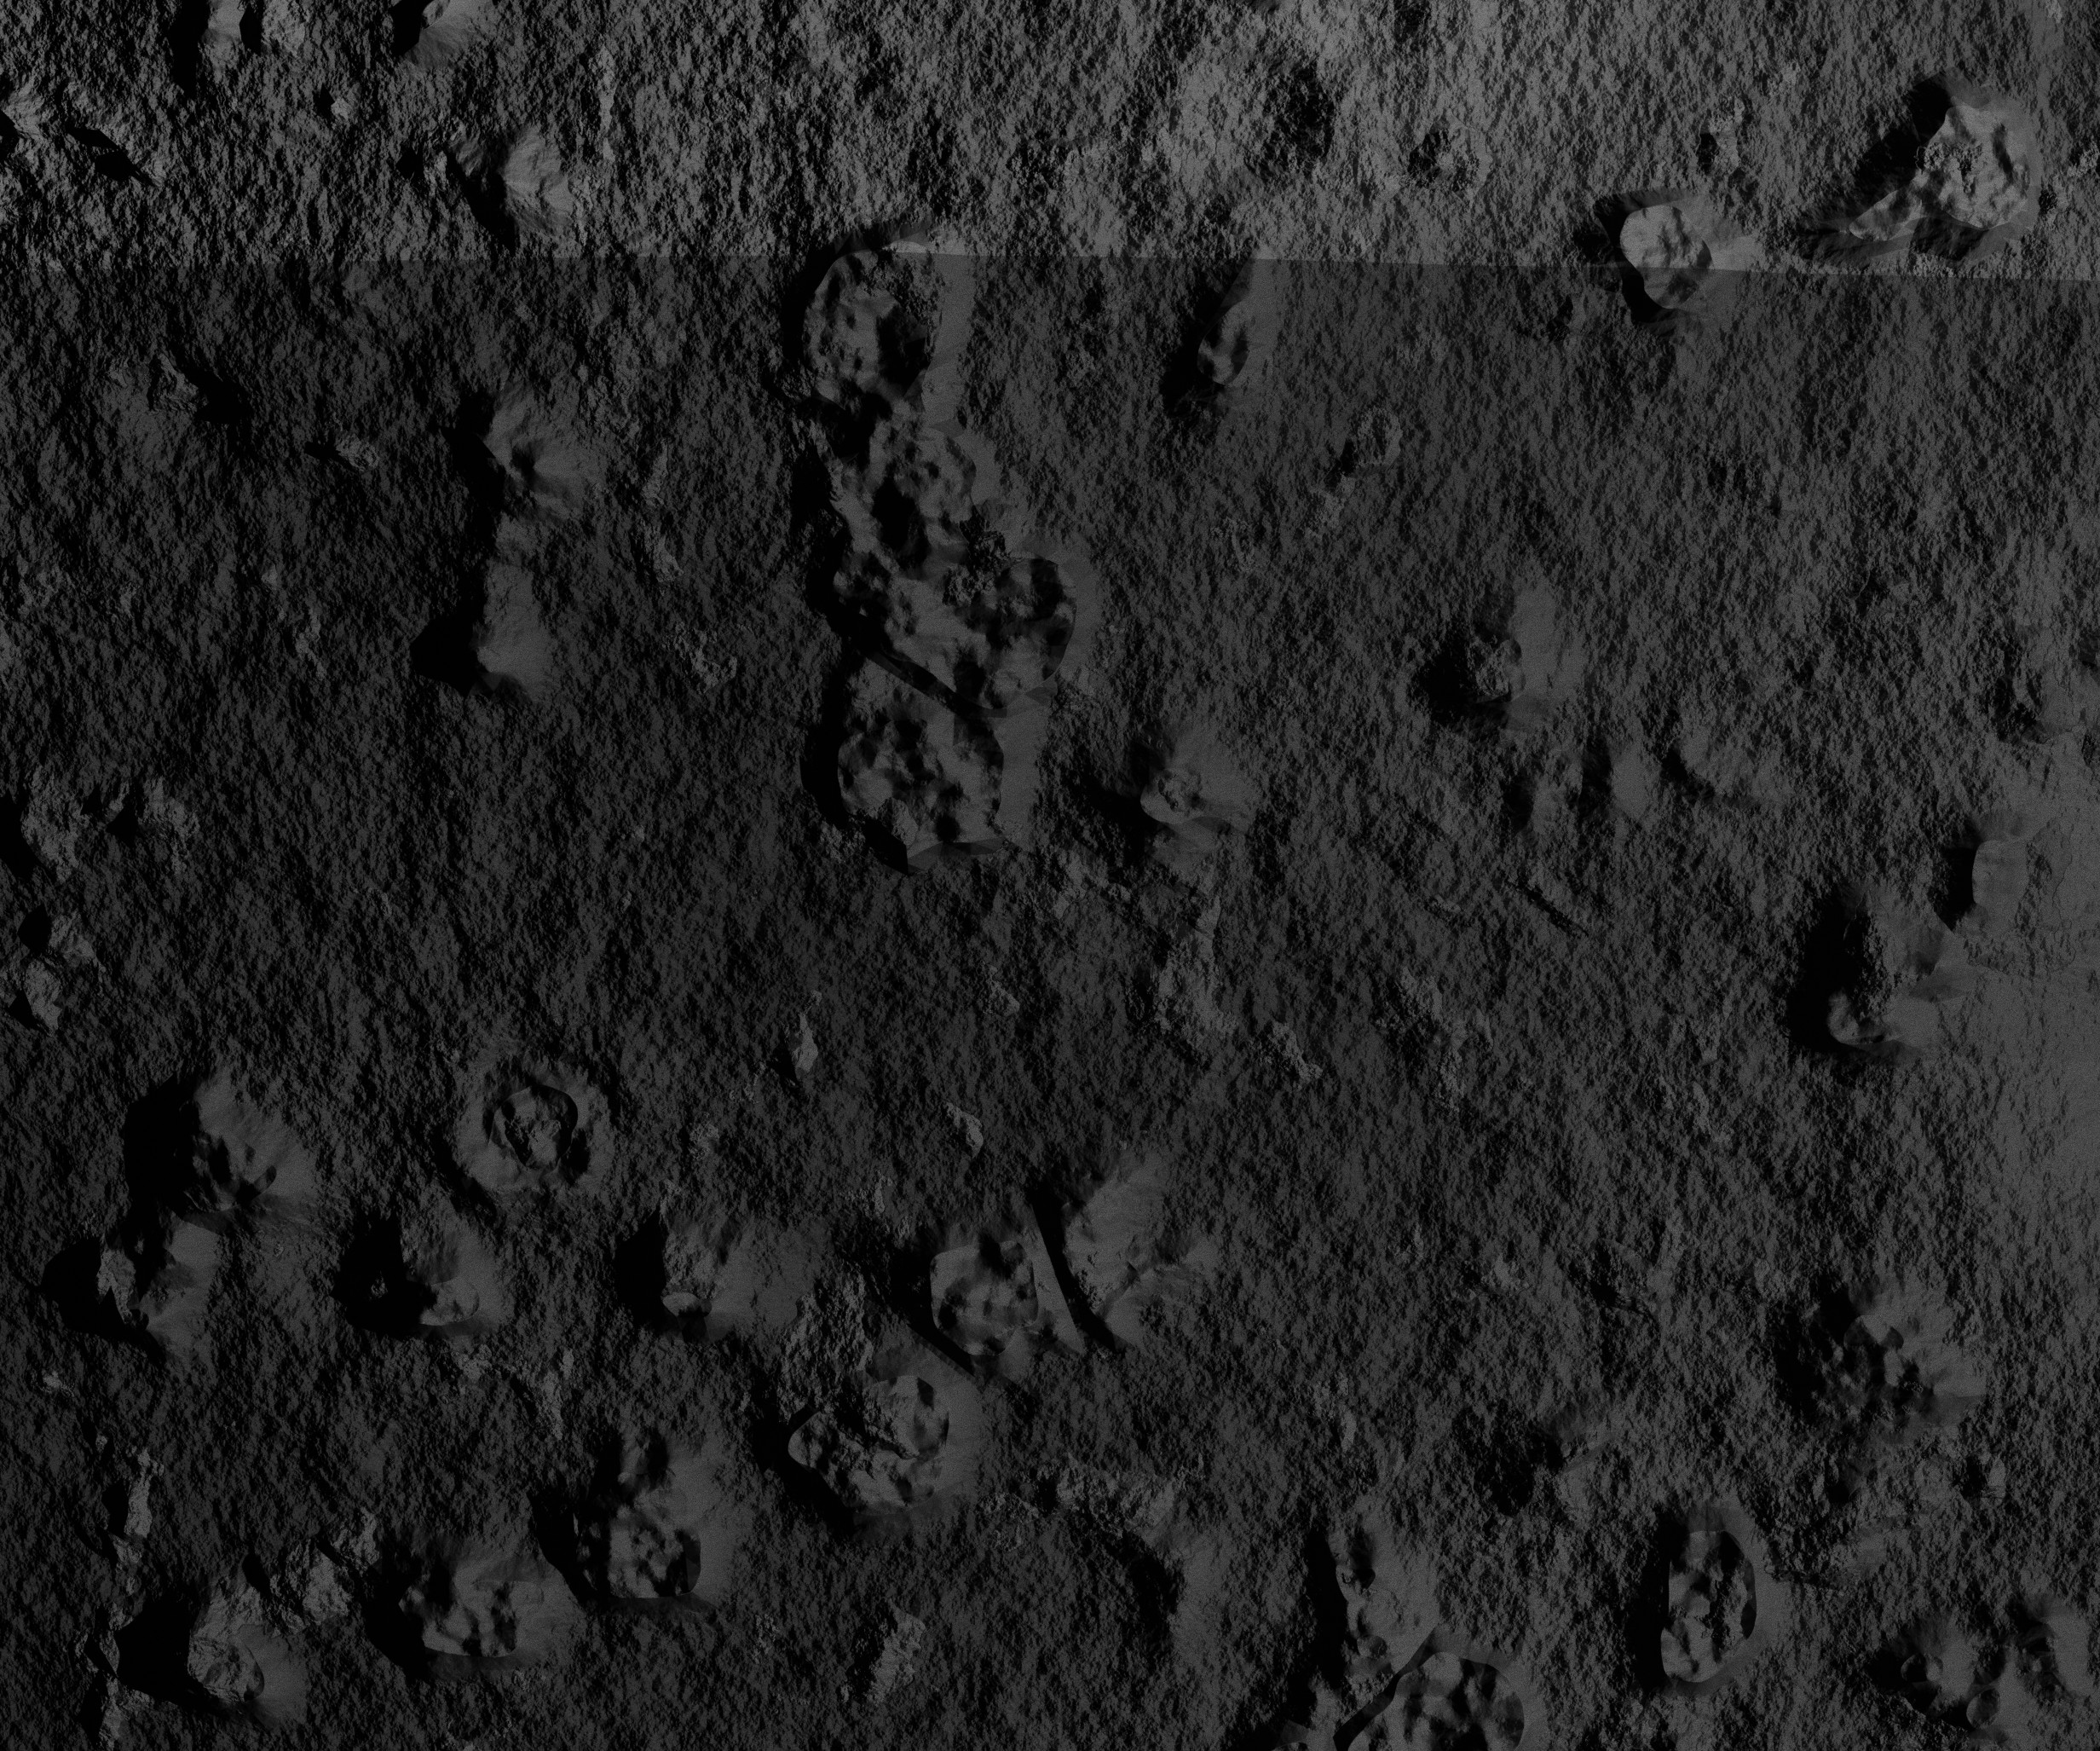
\includegraphics[width=\textwidth]{doc/thesis/0_figures/rendering_artefacts/50_10_SssbOnly_2017-08-15T115845-190000.jpg}
            \caption{\SI{50}{\kilo\meter}.}
            \label{fig:render_artefacts_50}
        \end{subfigure}
        \begin{subfigure}[b]{0.32\textwidth}
            \centering
            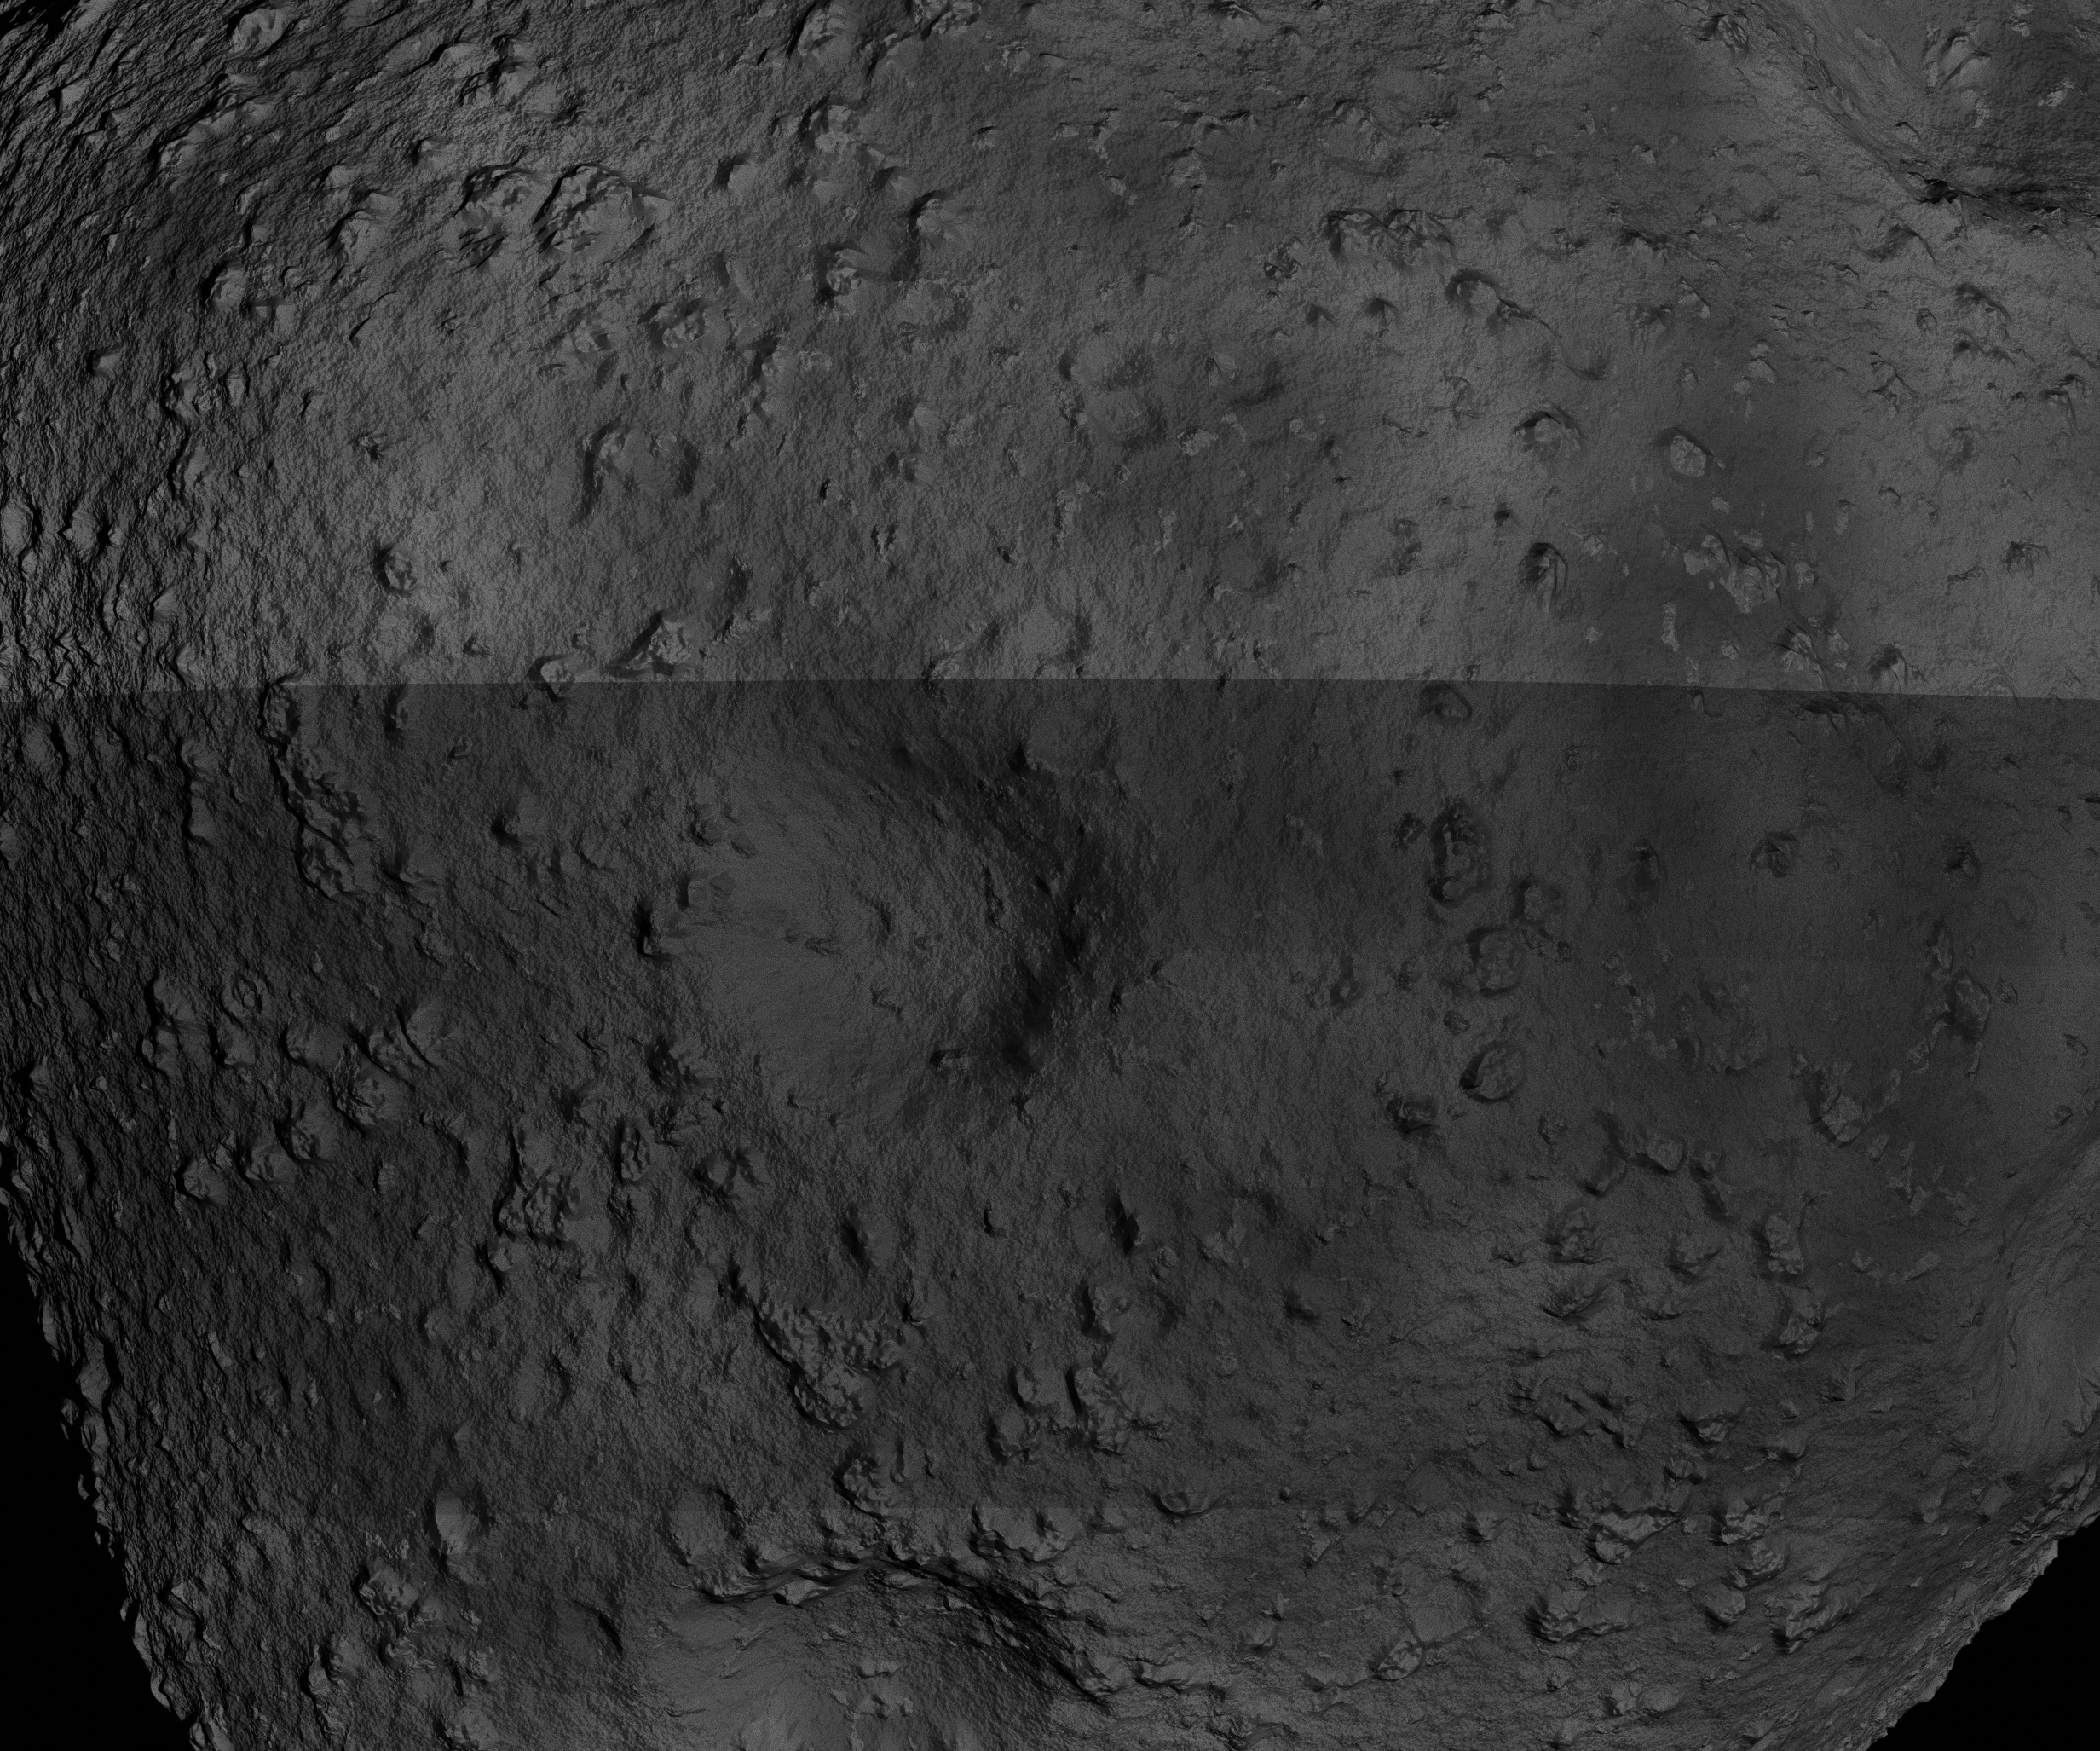
\includegraphics[width=\textwidth]{doc/thesis/0_figures/rendering_artefacts/200_10_SssbOnly_2017-08-15T115845-190000.jpg}
            \caption{\SI{200}{\kilo\meter}.}
            \label{fig:render_artefacts_200}
        \end{subfigure}
        \begin{subfigure}[b]{0.32\textwidth}
            \centering
            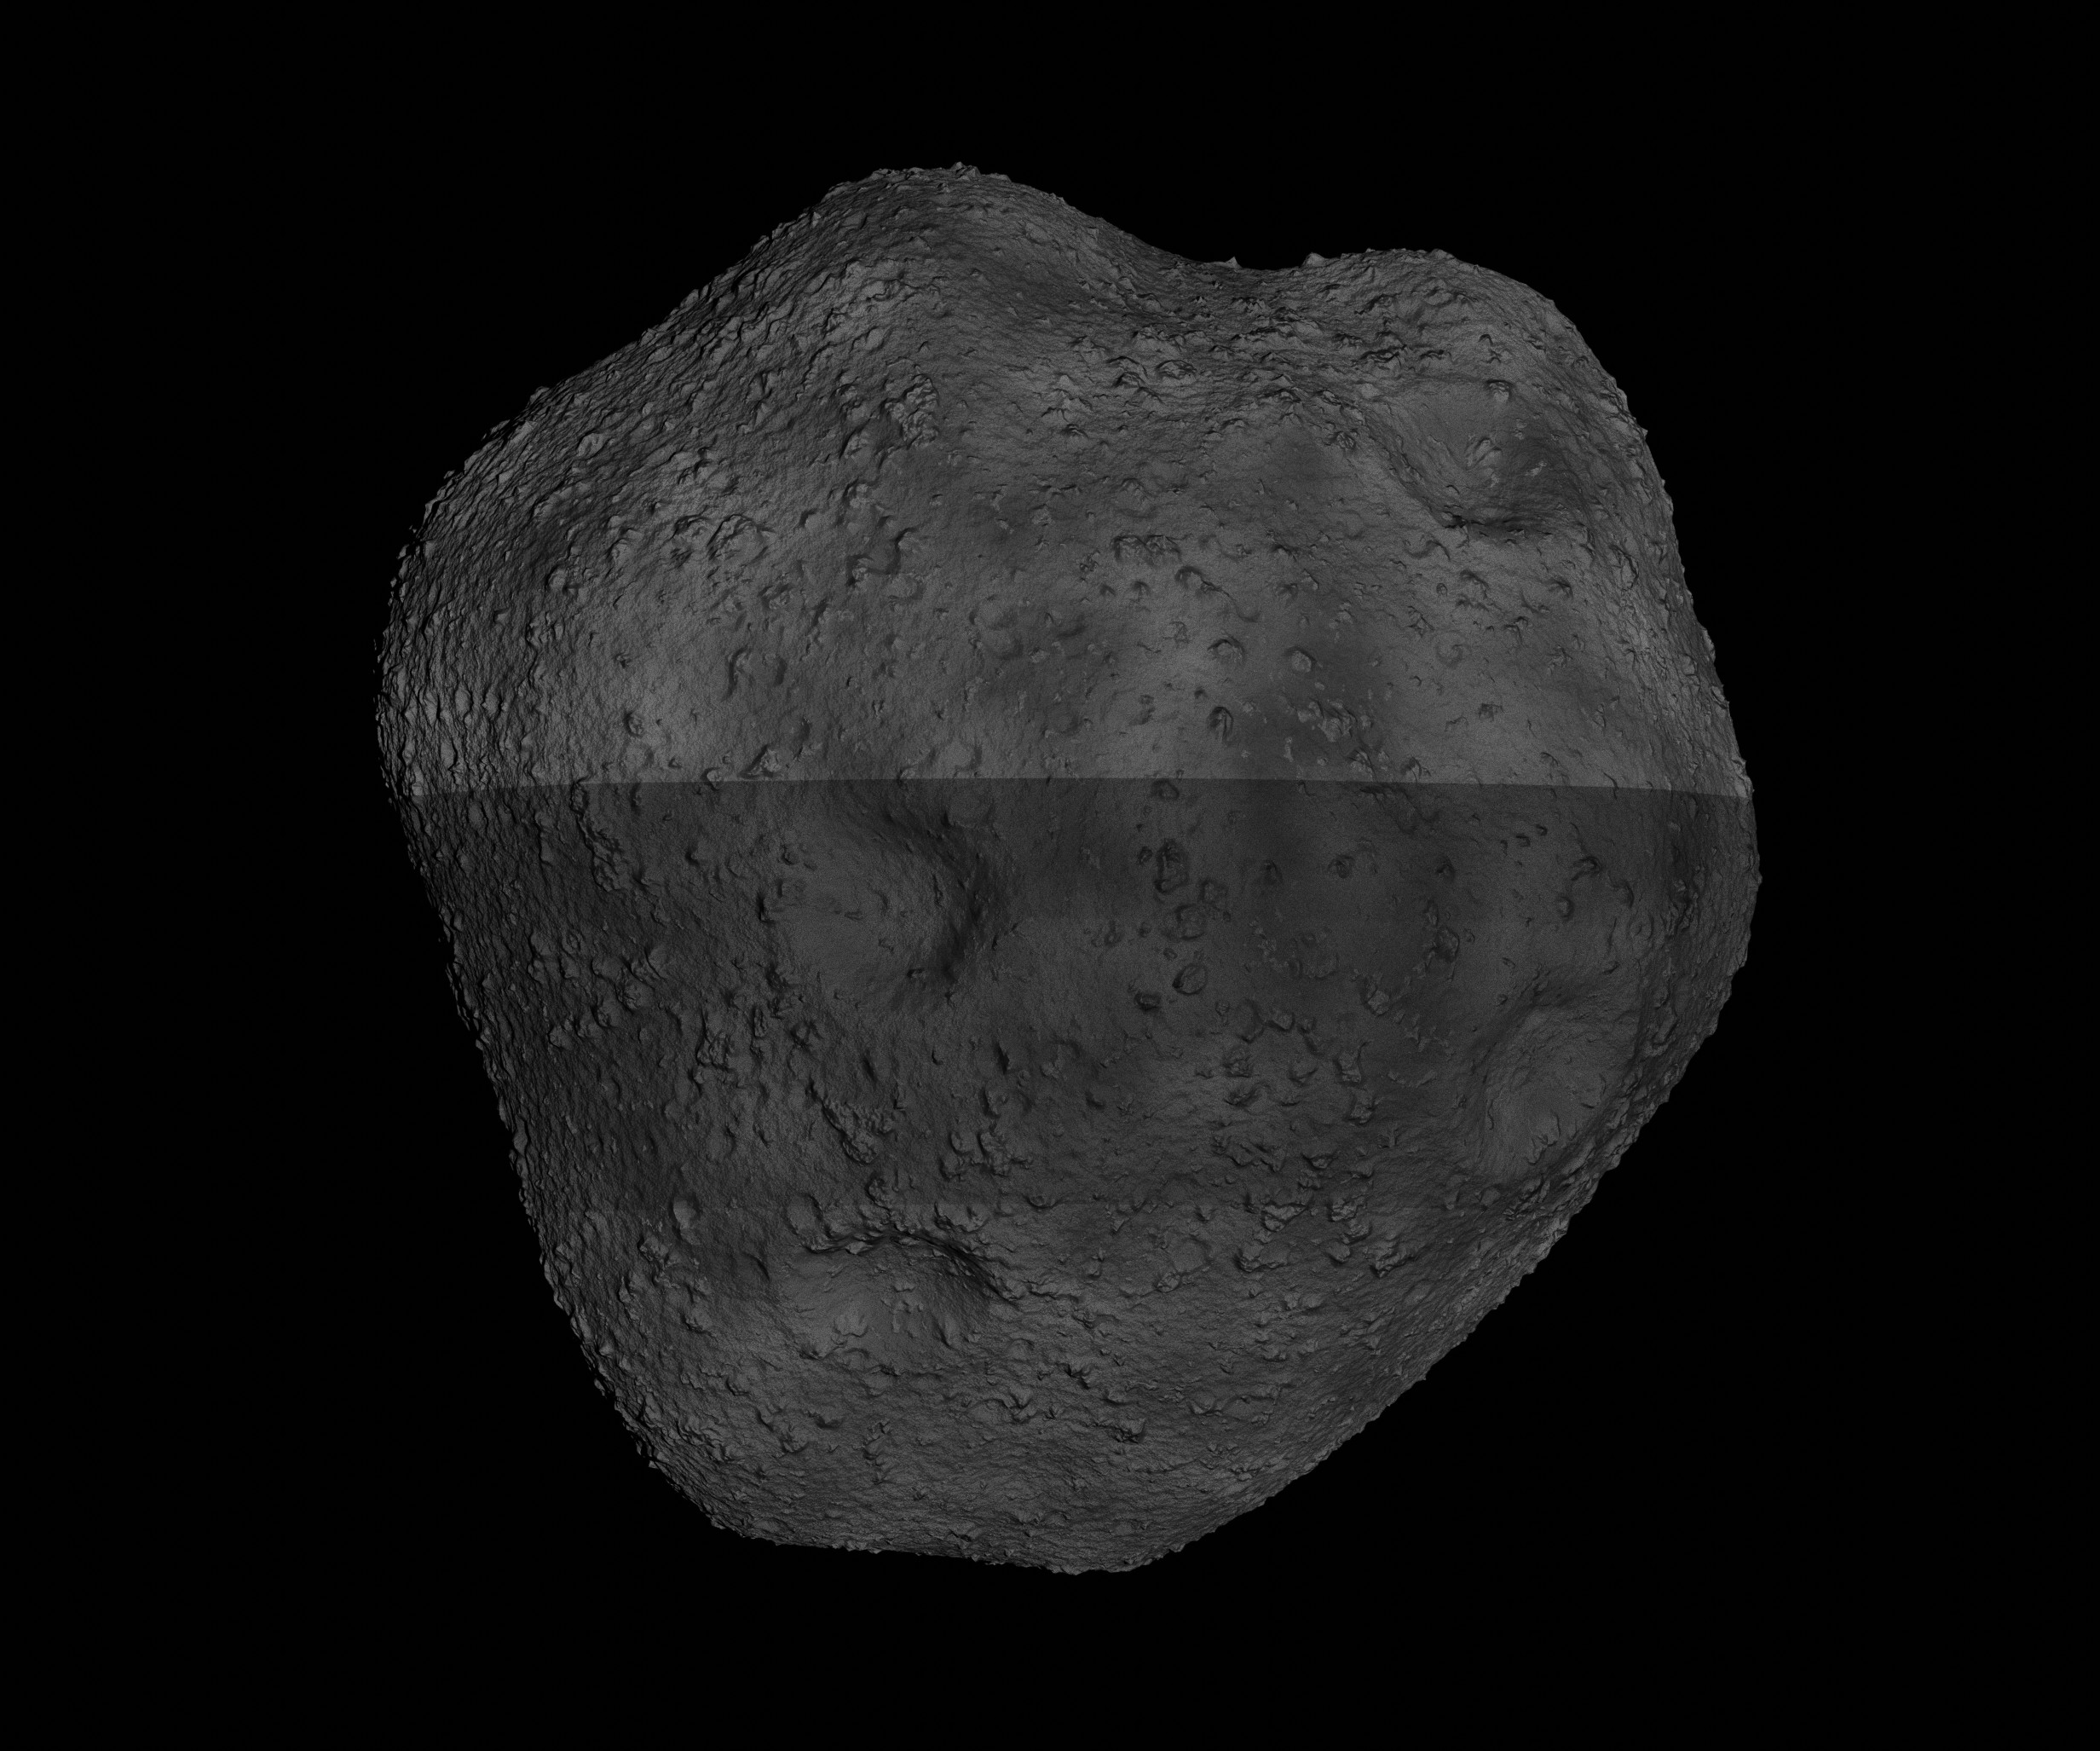
\includegraphics[width=\textwidth]{doc/thesis/0_figures/rendering_artefacts/400_10_SssbOnly_2017-08-15T115845-190000.jpg}
            \caption{\SI{400}{\kilo\meter}.}
            \label{fig:render_artefacts_400}
        \end{subfigure}
    \caption{Surface of a \SI{10}{\kilo\meter} \gls{sssb} for flybys with the given closest approach distance. Rendering artefacts, the stripes, are clearly visible in all three images.}
    \label{fig:render_artefacts}
\end{figure}

\subsection{Compression} \label{sec:results_comp}
The \gls{sispo} software package was used to study the effects of compression in different scenarios. The scenarios are presented in Table \ref{tab:sim_params}. Two compression algorithms were used to study compression effects. The \gls{png} format was used because of its wide support among different software packages and \gls{jpeg}2000. Scenarios with varying \gls{sssb} nucleus sizes and flyby distance were simulated. 
Comparison of the different compression algorithms is based on several output parameters. The data size of the compressed image series, the number of points in the dense reconstructed point cloud, the number of vertices and the number of faces of the refined reconstructed model. These outputs relate well to the level of detail of the rendered images, since \gls{sfm} algorithms rely on surface details for reconstruction.

\begin{table}[htb]
    \centering
    \caption{Simulation parameters used for investigating capabilities of \gls{sispo}. For each scenario \gls{png}, \gls{jp2} quality 1000, quality 100, quality 10 and quality 1 compression methods were used to investigate the effects of compression.}
    \label{tab:sim_params}
    \begin{tabular}{l|lll}
        ID      & \gls{sssb} Size \SI{}{\kilo\meter} & Encounter Distance \SI{}{\kilo\meter} & Number of Images \\ \hline
        Default & 1  & 50  & 120\\
        Default & 1  & 100 & 120\\
        Default & 1  & 200 & 120\\
        Default & 1  & 400 & 120\\
        Default & 1  & 50  & 30\\
        Default & 1  & 100 & 30\\
        Default & 1  & 200 & 30\\
        Default & 1  & 400 & 30\\
        Default & 10 & 50  & 30\\
    \end{tabular}
\end{table}

\subsubsection{Image Quality Comparison}
To compare the image quality after different levels of compression, a specific image is selected which is compressed to different levels. Since reconstruction is mostly influenced by surface features, a scene with a distance of \SI{50}{\kilo\meter} was selected for comparison. To better show the artefacts created by compression, the highlighted area in Figure \ref{fig:img_quality_frame} was studied up closer.

\begin{figure}[htb]
    \centering
    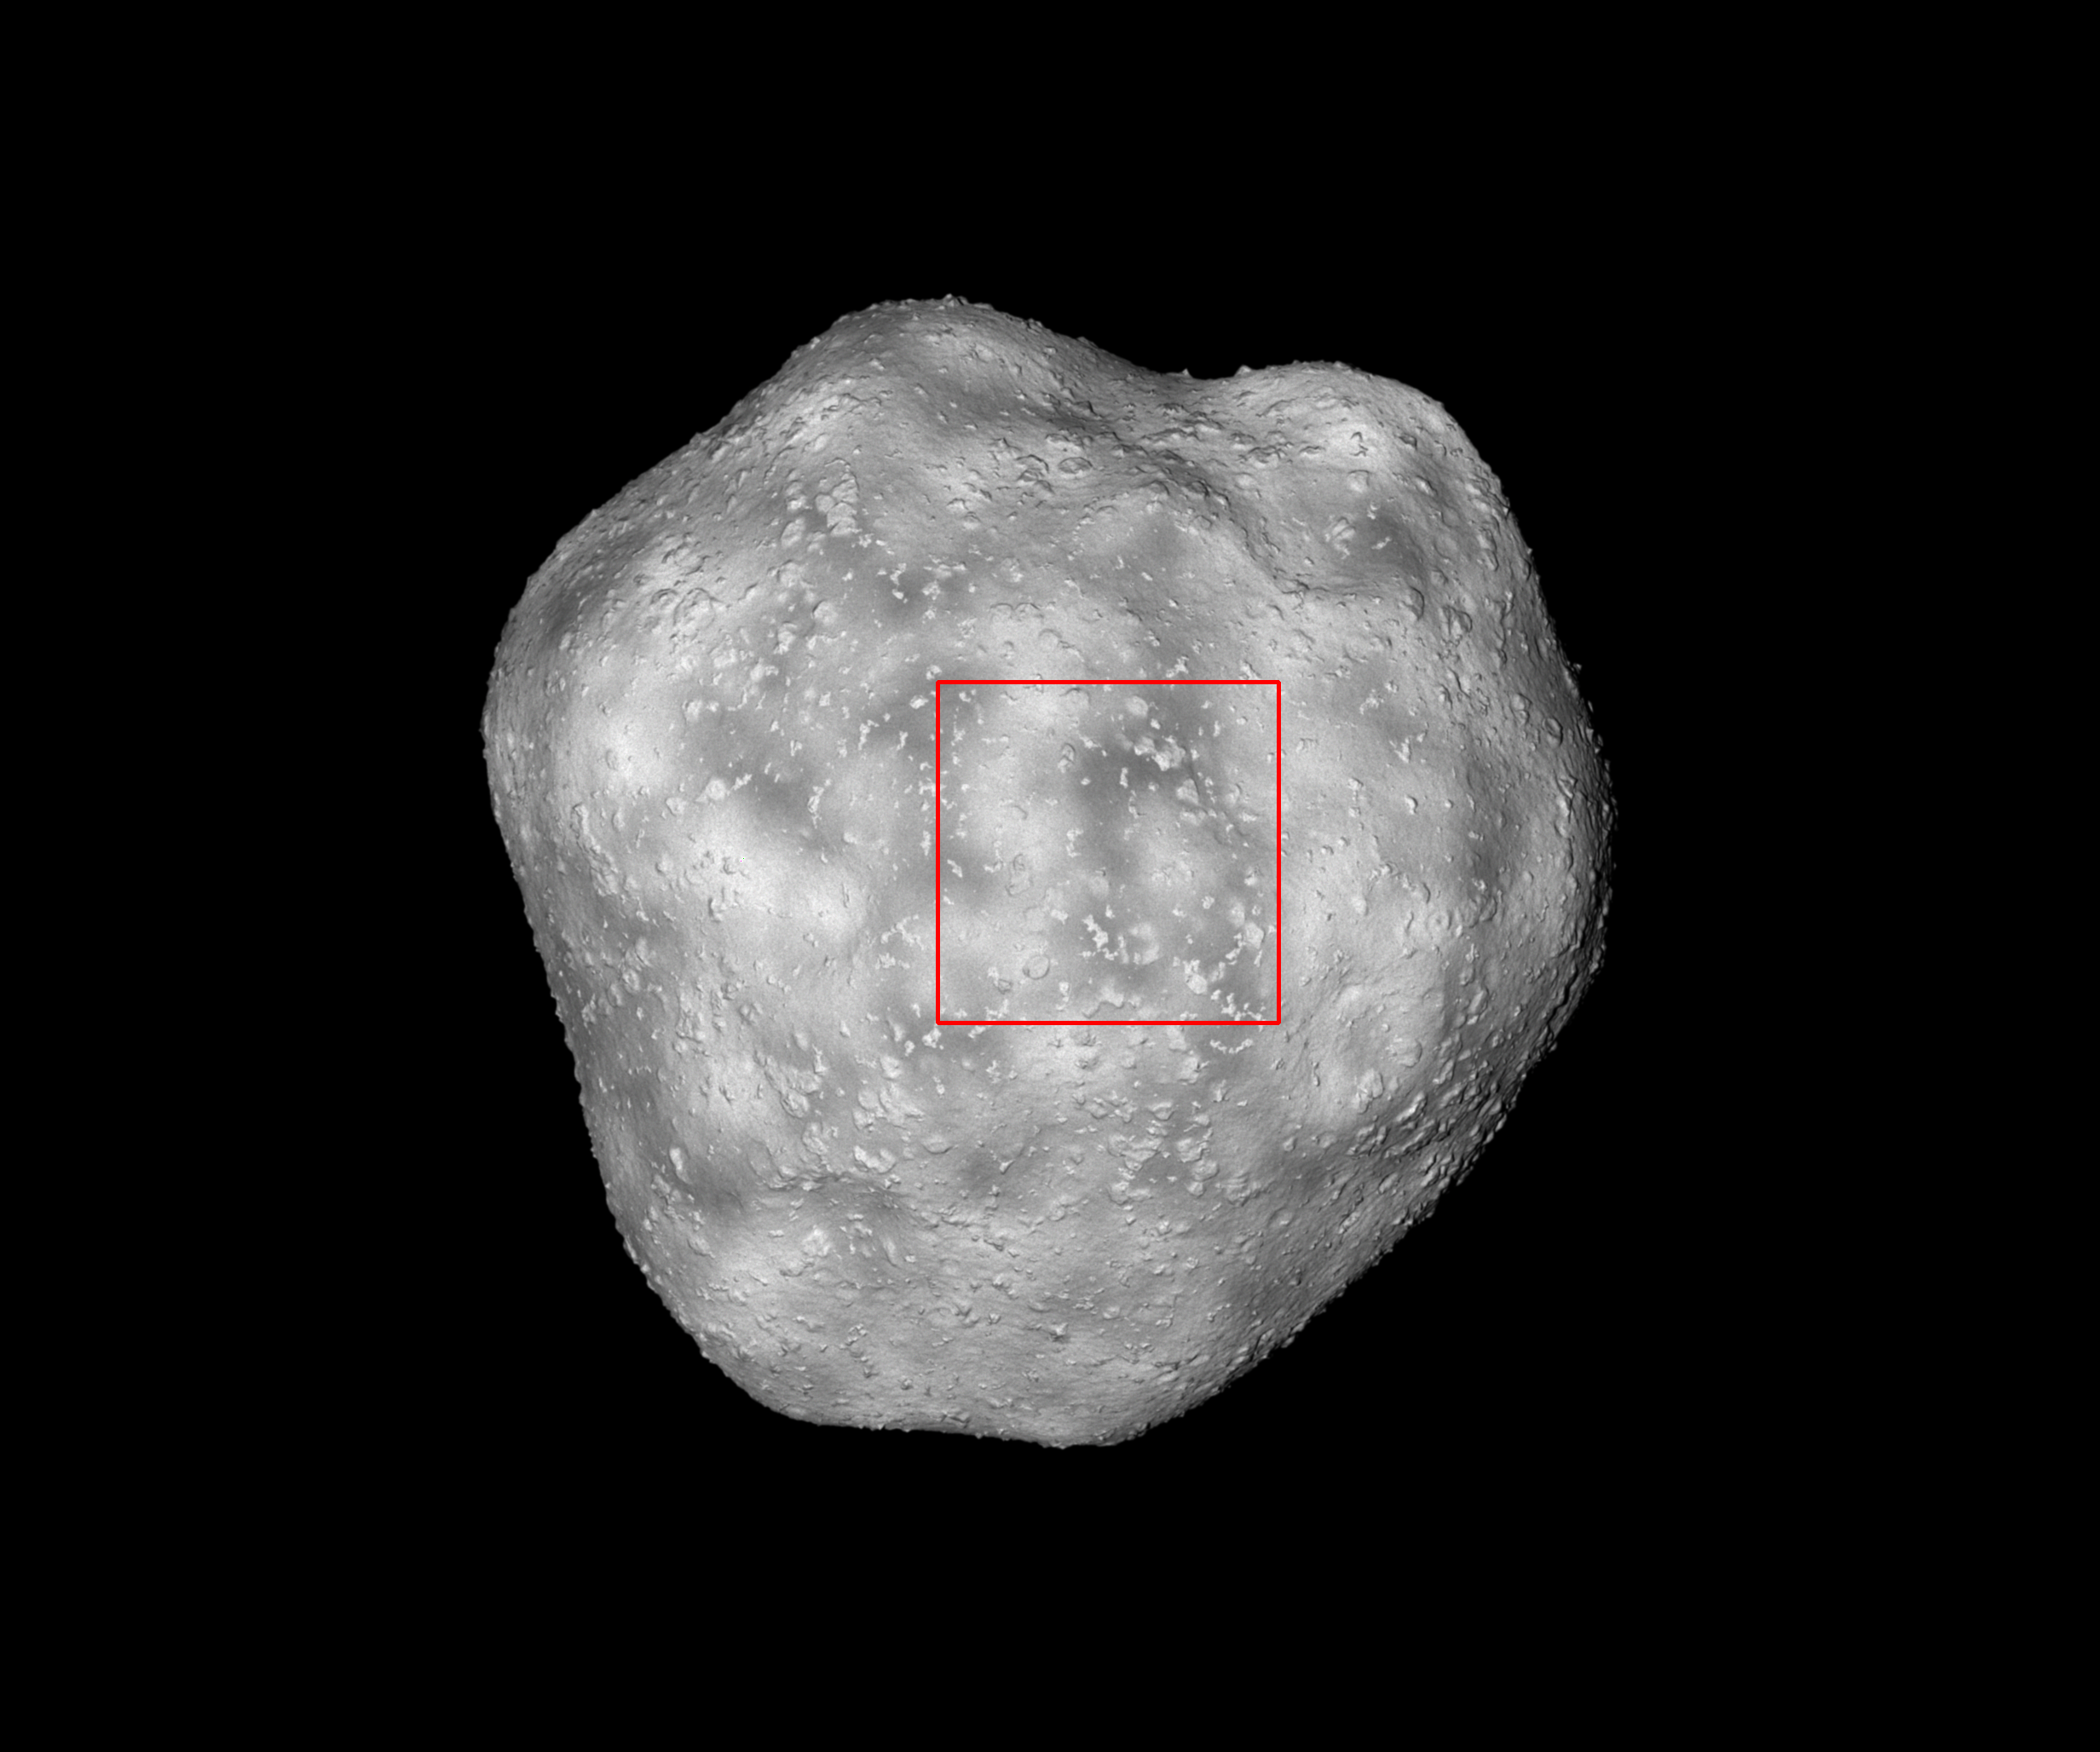
\includegraphics[width=.7\textwidth]{doc/thesis/0_figures/quality_compare/jp2_1000_frame.png}
    \caption{Scene used for quality comparison. Highlighted in red is the area studied up closer. The specific area was selected since it includes a wide range of colours and various sized surface features.}
    \label{fig:img_quality_frame}
\end{figure}

Figure \ref{fig:img_quality_comp} shows series of close-up views of rendered images at different levels of compression. At higher quality levels only few samples are shown since the differences are small.

\begin{figure}[htb]
    \centering
        \begin{subfigure}[b]{0.47\textwidth}
            \centering
            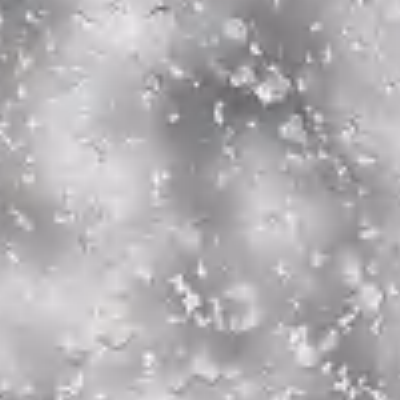
\includegraphics[width=\textwidth]{doc/thesis/0_figures/quality_compare/jp2_1_center.png}
            \caption{Quality 1.}
            \label{fig:img_quality_1}
        \end{subfigure}
        \begin{subfigure}[b]{0.47\textwidth}
            \centering
            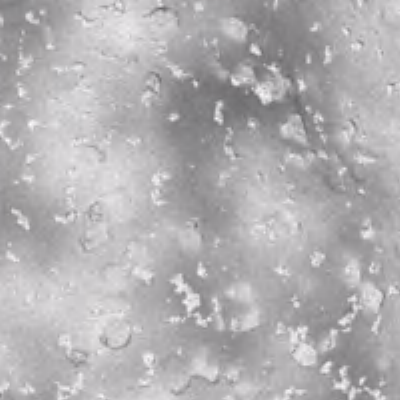
\includegraphics[width=\textwidth]{doc/thesis/0_figures/quality_compare/jp2_4_center.png}
            \caption{Quality 4.}
            \label{fig:img_quality_4}
        \end{subfigure}
        \\
        \begin{subfigure}[b]{0.47\textwidth}
            \centering
            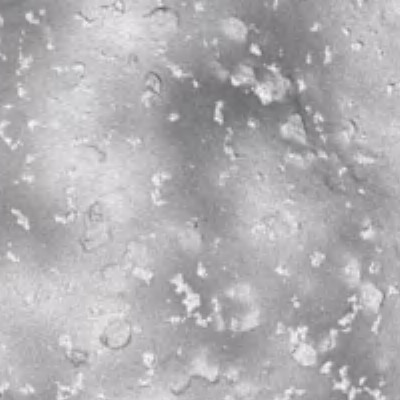
\includegraphics[width=\textwidth]{doc/thesis/0_figures/quality_compare/jp2_5_center.png}
            \caption{Quality 5.}
            \label{fig:img_quality_5}
        \end{subfigure}
        \begin{subfigure}[b]{0.47\textwidth}
            \centering
            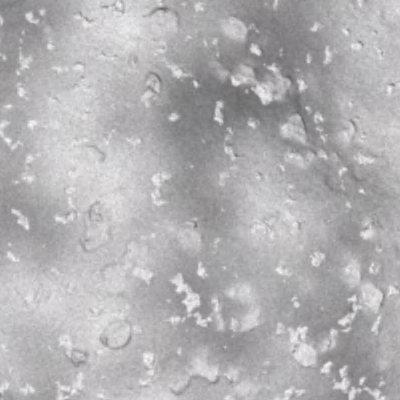
\includegraphics[width=\textwidth]{doc/thesis/0_figures/quality_compare/jp2_10_center.png}
            \caption{Quality 10.}
            \label{fig:img_quality_10}
        \end{subfigure}
        \\
        \begin{subfigure}[b]{0.47\textwidth}
            \centering
            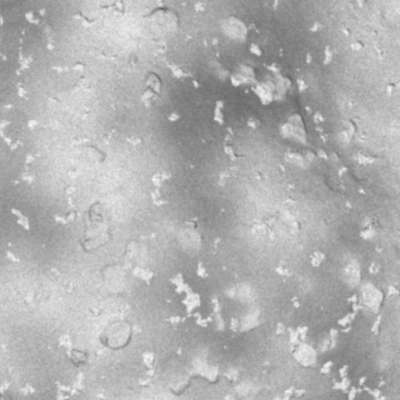
\includegraphics[width=\textwidth]{doc/thesis/0_figures/quality_compare/jp2_100_center.png}
            \caption{Quality 100.}
            \label{fig:img_quality_100}
        \end{subfigure}
        \begin{subfigure}[b]{0.47\textwidth}
            \centering
            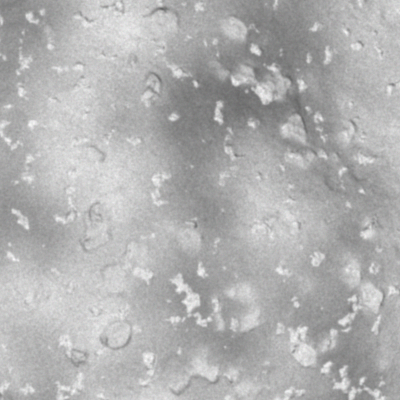
\includegraphics[width=\textwidth]{doc/thesis/0_figures/quality_compare/jp2_1000_center.png}
            \caption{Quality 1000.}
            \label{fig:img_quality_1000}
        \end{subfigure}
    \caption{Comparison of images with different level of compression using \gls{jpeg}2000.}
    \label{fig:img_quality_comp}
\end{figure}

Visual comparison of the different images reveals that quality 1000 is indistinguishable from quality 100. Also quality 10 resembles quality 1000 quite well. When comparing quality 5 to quality 1000 the images are still similar though quality 5 looks blurred. When looking at the quality 1 image, the overall surface colouring and main surface features are still visible. However, compression artefacts become strongly visible.

\subsection{Reconstruction}
\gls{sispo} is choosing which result of which reconstruction method to use based on the number of reconstructed points. Comparing the chosen algorithm with the input parameter reveals that the first incremental \gls{sfm} reconstruction performs better when the flyby distance is smaller while the second incremental \gls{sfm} algorithms performs better with farther flyby distances.

\begin{table}[htb]
    \centering
    \caption{Reconstruction Settings}
    \label{tab:comp_settings}
    \begin{tabular}{l|l}
        \textbf{Parameter Name} & \textbf{Value} \\ \hline
        export\_type       & obj   \\
        focal & 66667 \\
        cam\_model & \SI{1}{}     \\
        geo\_model & \SI{10}{\kilo\meter\per\second} \\
        num\_overlaps  & \SI{4}{} \\
        use\_prior & \SI{1}{} \\
        use\_upright & \SI{0}{} \\
        force\_compute & \SI{0}{} \\
        descriptor & SIFT \\
        d\_preset & ULTRA \\
        method & FASTCASCADEHASHINGL2 \\
        refine\_options & NONE \\
        reduce\_memory & 1
    \end{tabular}
\end{table}

\subsubsection{Reconstructed Model Comparison}
Several models were reconstructed etc.

Number of reconstructed points increases with increasing \gls{sssb} size and decreasing encounter distance.


\subsubsection{Reconstruction Limits}
Reconstructing the \gls{sssb} nucleus for a range of flyby scenarios allows to show some of the limits of the reconstruction pipeline.

Closer seems not to be a problem, farther away means less and less features. \SI{400}{\kilo\meter} worked with \SI{1}{\kilo\meter} \gls{sssb}. 
\SI{0.1}{\kilo\meter} worked until \SI{100}{\kilo\meter} closest approach.


\subsubsection{Reconstruction Algorithms}
Since \gls{sispo} uses three different \gls{sfm} algorithms, it is investigated which algorithm is most successful under which parameter set.

While the global \gls{sfm} algorithm was able to reconstruct a point cloud in various cases, it never created the best output. The number of points in the reconstructed point cloud of the incremental \gls{sfm} algorithms always exceeded those of the global \gls{sfm} algorithm.

\subsection{Overall Performance}
\gls{sispo} was executed on a machine running Linux Ubuntu 18.04.03 LTS, \SI{16}{\giga\byte} of \gls{ram}, Intel\textsuperscript{\textregistered}~Core\texttrademark~i7-8700 processor with \SI{6}{} cores and an NVIDIA\textsuperscript{\textregistered}~GeForce GTX 1080 with \SI{8}{\giga\byte} memory. The performance assessment of a complete \gls{sispo} run shows that the most time consuming part is rendering. 
A test case with an encounter distance of \SI{50}{\kilo\meter}, a relative velocity of \SI{30}{\kilo\meter\per\second} and \SI{120}{} images is investigated. The complete statistics are presented in Appendix \ref{sec:app_performance}. The total execution time is \SI{41849.938}{\second}. The time spent rendering is \SI{40617.382}{\second}, approximately \SI{97}{\percent} of the overall total. The time spent reconstructing was \SI{785.949}{\second}, approximately \SI{2}{\percent} of the overall total. Hence, the Python code was not improved to reduce execution time since \SI{99}{\percent} of the execution time stem from time spent outside the Python code.